% !TeX encoding = UTF-8
% !TeX root = ../thuthesis-example.tex

\chapter{基于2D-3D的图像-激光跨模态匹配定位}
\label{ch4}
\section{引言}
高精度离线地图的构建是复杂的,需要高精度的仪器设备对场景进行数据采集,并对点云进行配准,利用上一章的算法,能够由粗到精地对点云进行很好的对齐,得到的稠密点云地图,该地图能够包含更多的特征,为在场景中的智能体的定位提供更多的参照。

本章旨在解决通过视觉方式实现在先验场景中的定位问题,这需要
建立其2D与3D模态之间的匹配。但是,如图\ref{2d-and-3d}所示,平面图像之间与点云之间的特征能够分别建立统一的关系,实现查找和匹配,但图像与点云的点由于在模态和外观上存在巨大的差异,无法构建一个统一的描述子,因此难以进行直接匹配\cite{piasco2018survey}。
\begin{figure}
	\centering
	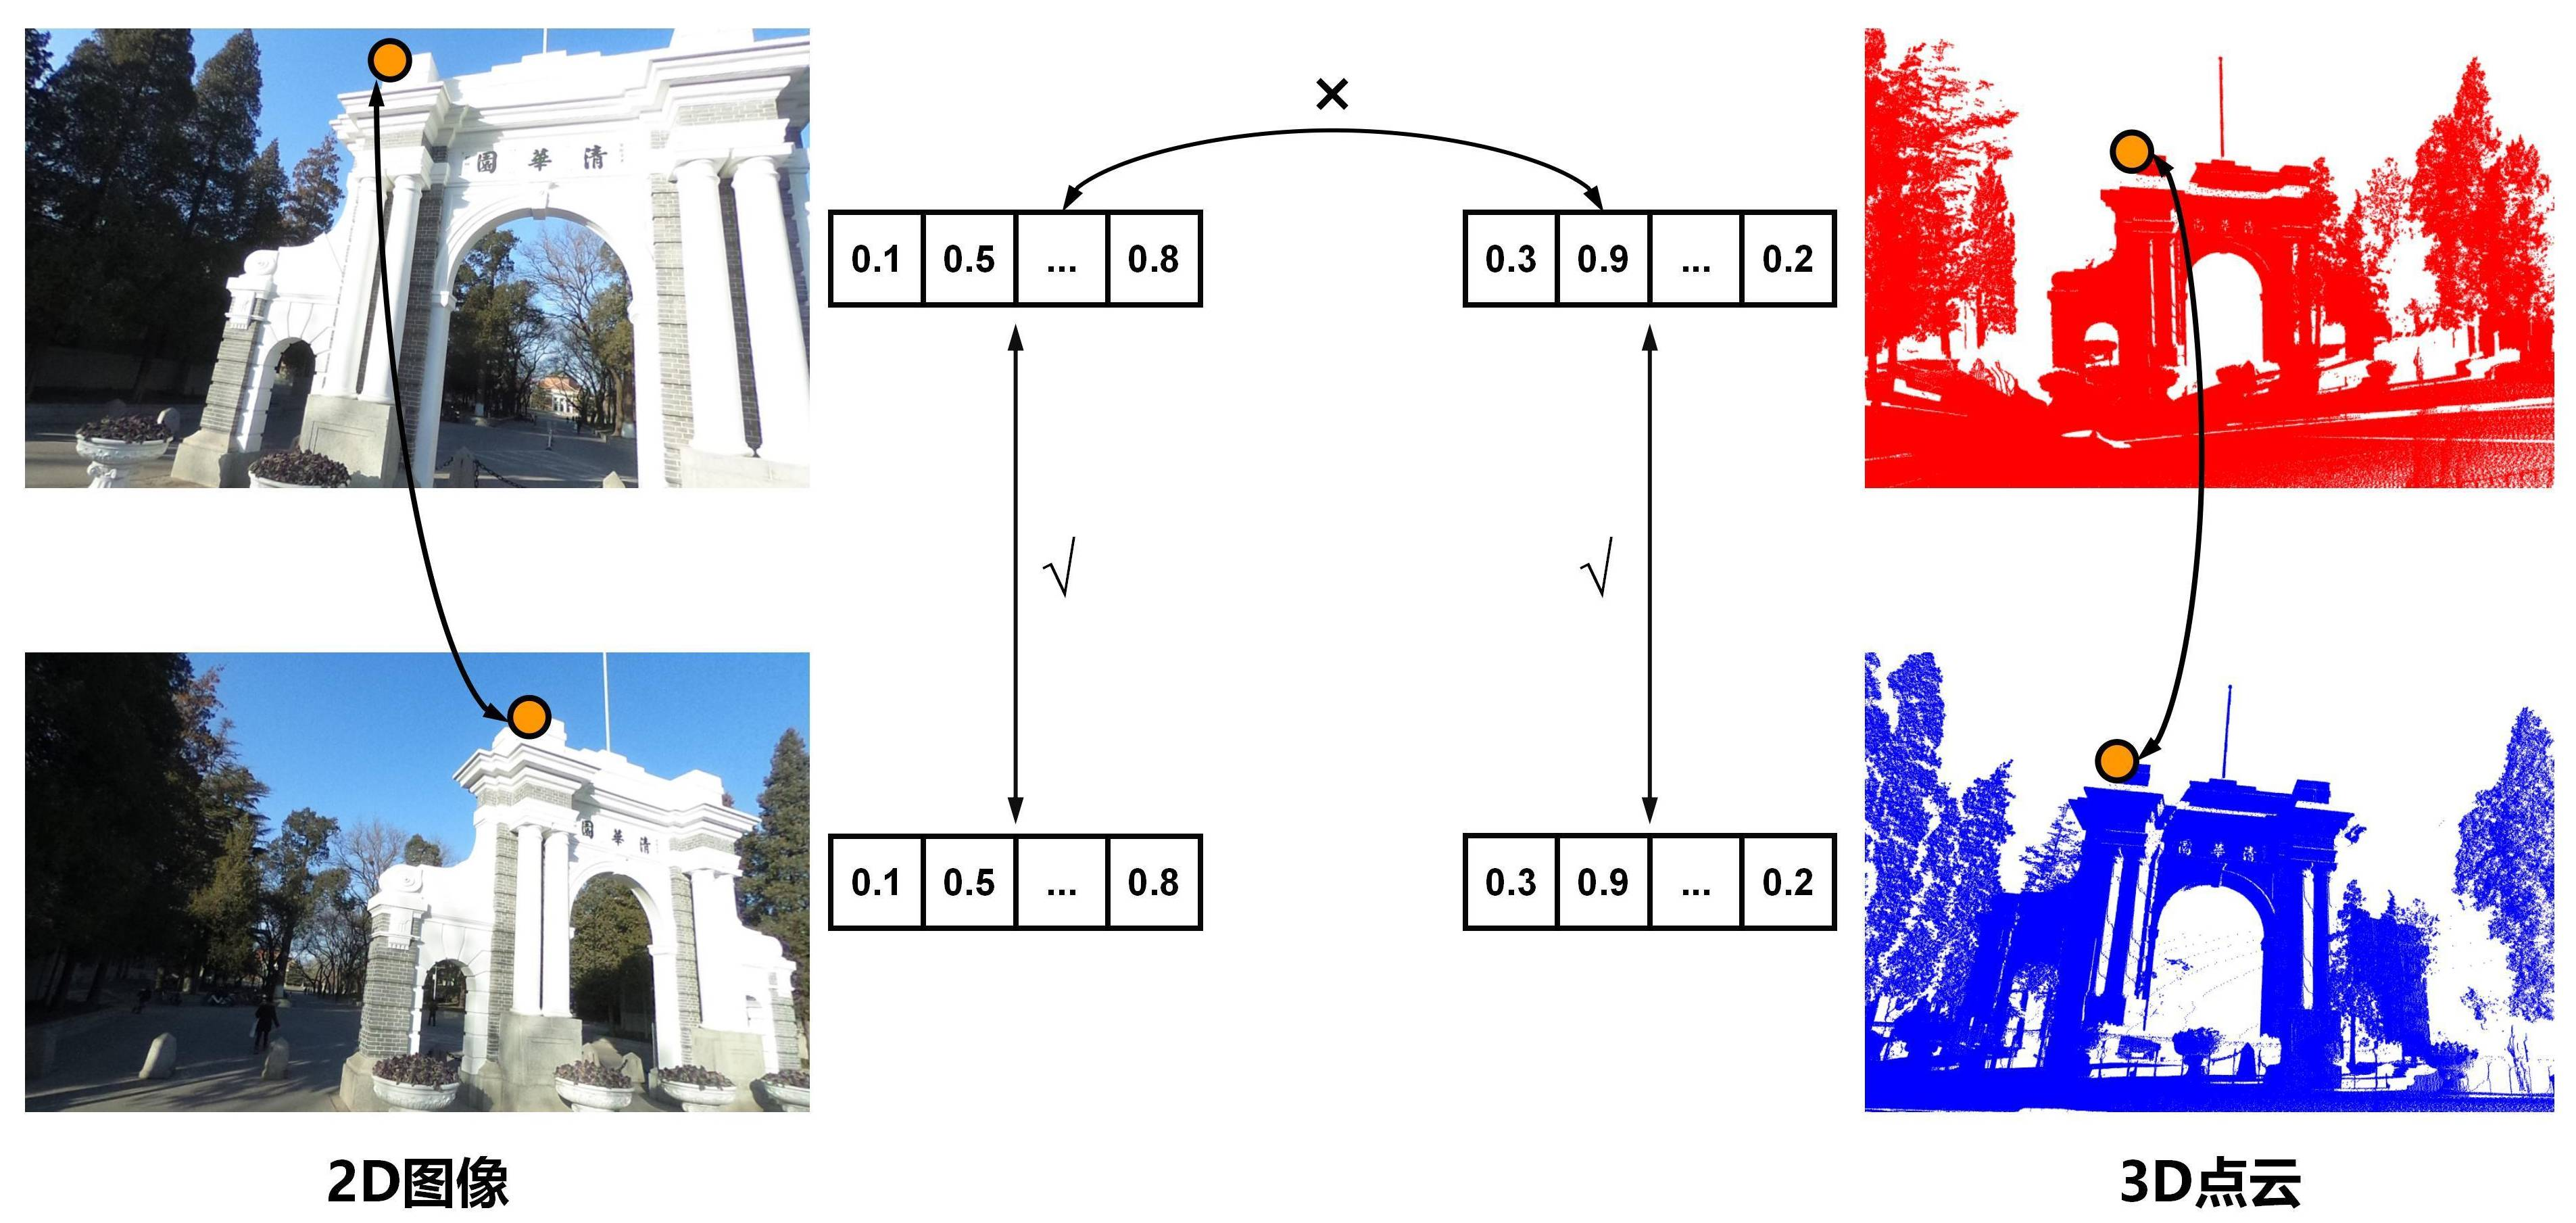
\includegraphics[width=14.5cm]{2d-and-3d}
	\caption{2D图像特征匹配与3D点云特征匹配}
	\label{2d-and-3d}
\end{figure}

本章针对这一挑战提出了一个流程,将难以直接匹配的2D-3D问题转化为2D-2D匹配问题。该算法的流程如图\ref{local-flowchart}所示,离线地图中储存了每个点的xyzrgb信息,可以先通过采用虚拟相机成像的方法,将场景的点投影到空间中的某一有限平面上,模拟在场景中的某一位置以若干视角拍摄的照片,这一步完成的是从3D点云到2D图像的转换。利用全景相机可以拥有到更广阔的视野,并且相比于激光雷达可以获取环境中的颜色信息,因此在本算法中被用作定位设备。但全景相机需要进行畸变校正,故首先对拍摄的全景图像进行切分校正,然后在两个图像对之间,利用基于深度学习的SOS-Net\cite{tian2019sosnet}进行鲁棒的特征点匹配,最后利用对极几何的方法求得2D图片与场景中某一已知位置之间的转移矩阵,从而实现定位的目的。
\begin{figure}
	\centering
	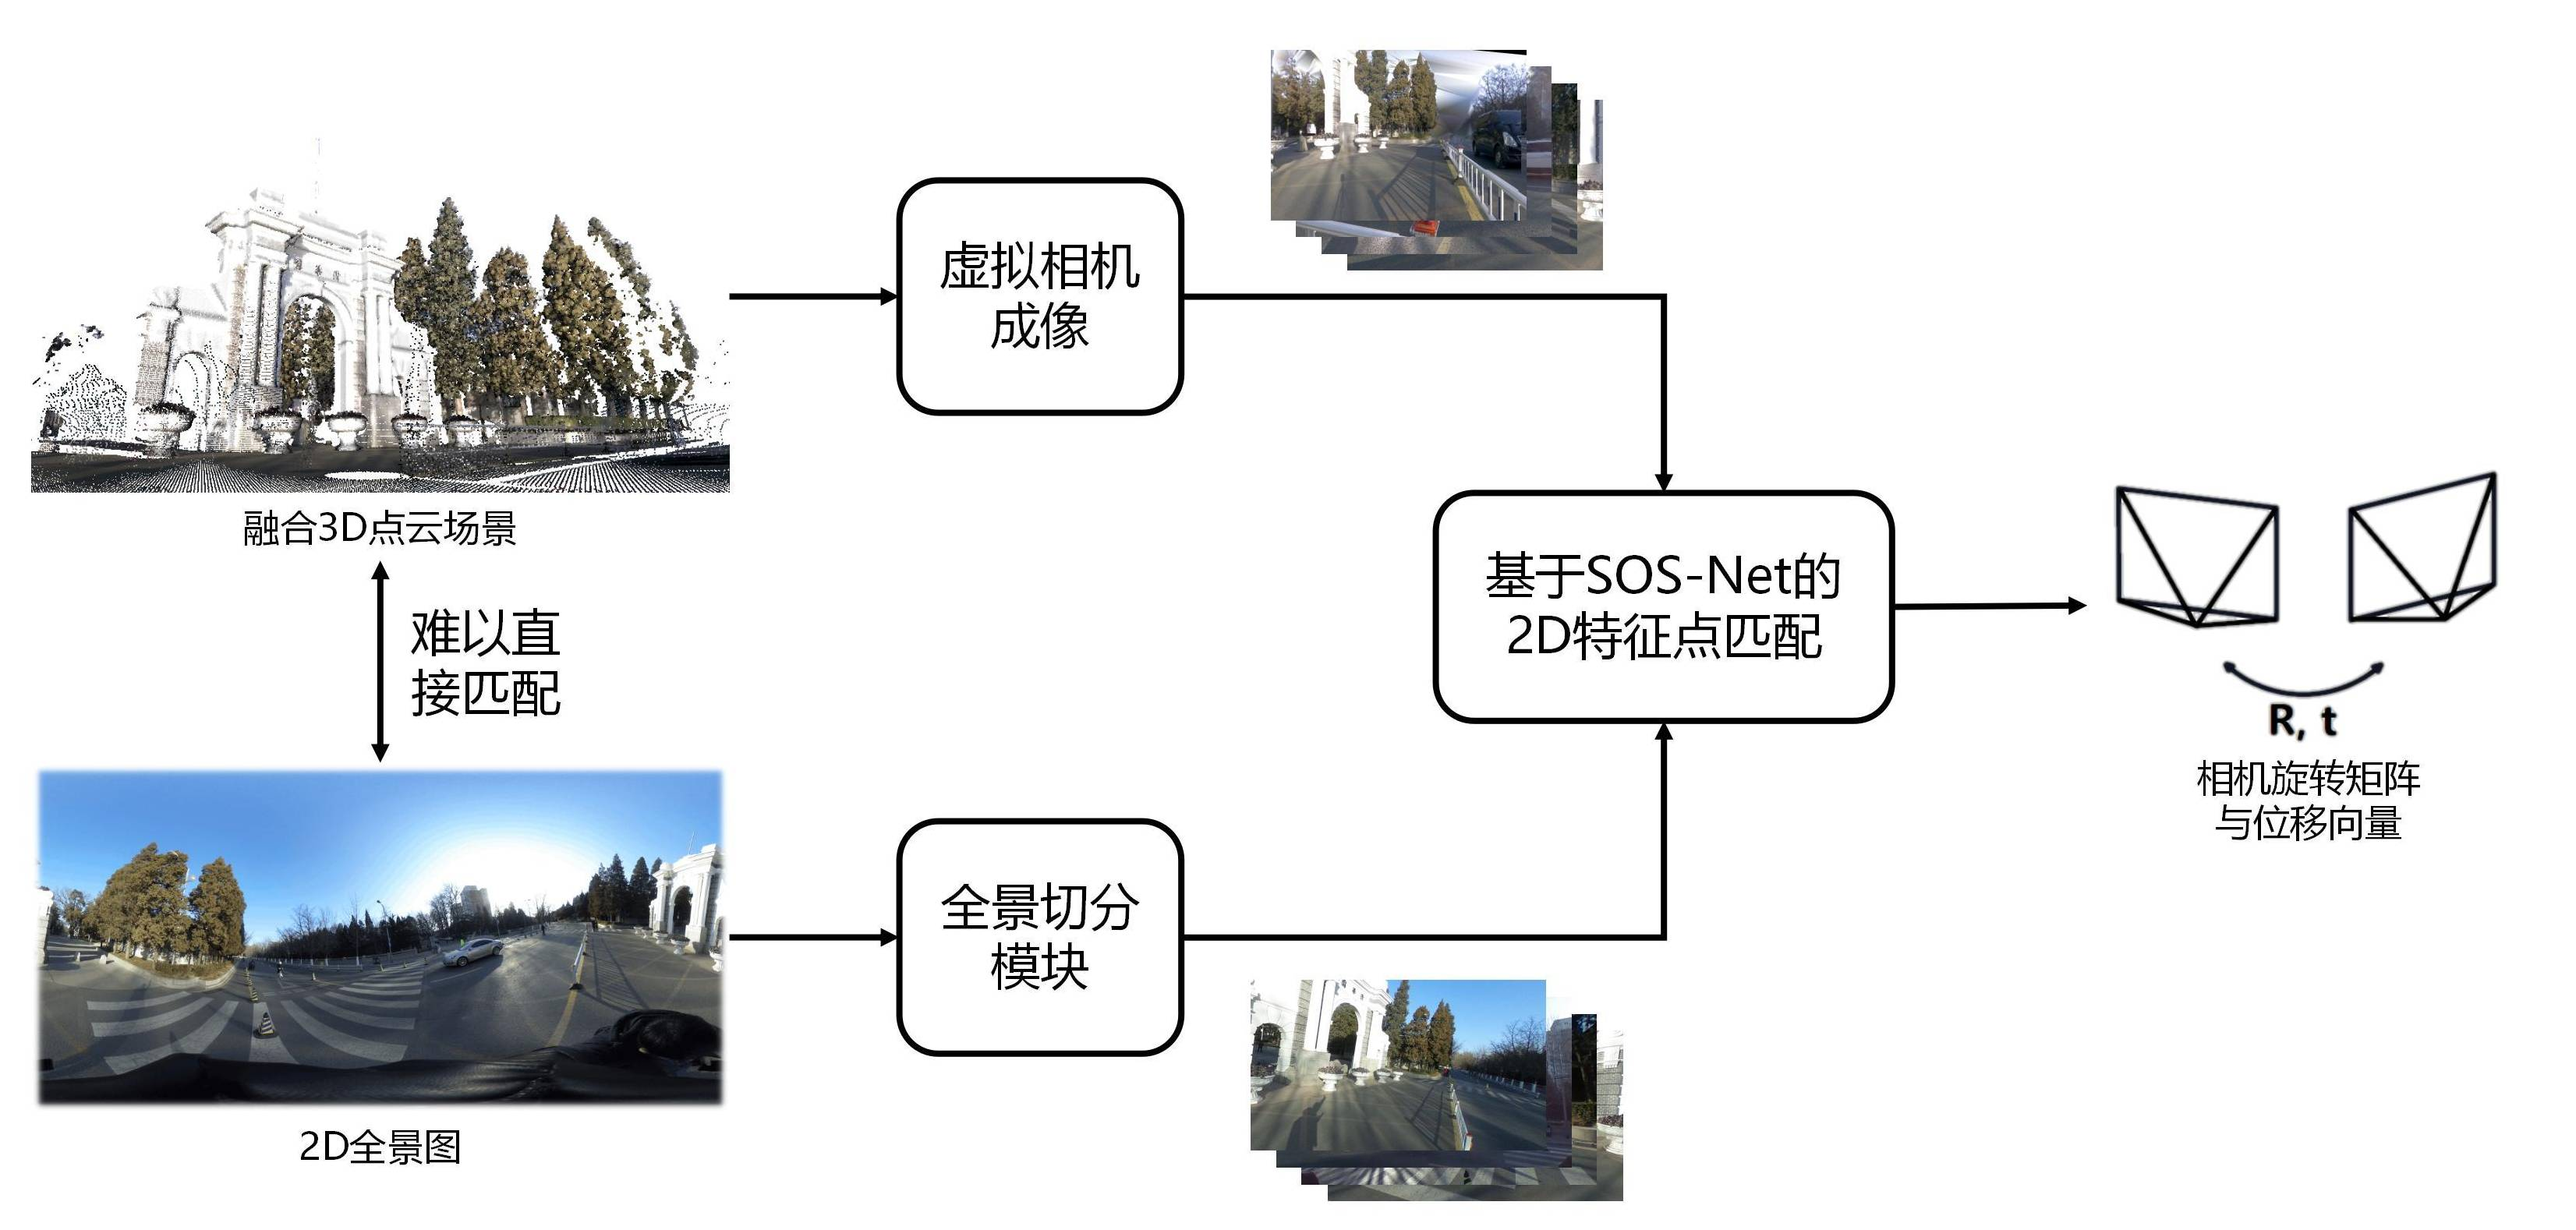
\includegraphics[width=14.5cm]{local-flowchart}
	\caption{基于2D-3D匹配的高精度点云场景定位算法流程图}
	\label{local-flowchart}
\end{figure}

\section{点云-平面映射}
\label{point-cloud-to-plane}
\subsection{虚拟视点图像生成}
相机能够将从真实三维世界中获取点的颜色信息,并将其投影到胶片上,将三维世界的点转变为平面上点的过程被称为相机模型。本文采用了最简单针孔相机模型,将点云图像中的点投影到给定虚拟视点和虚拟成像平面上。

\begin{figure}
	\centering
	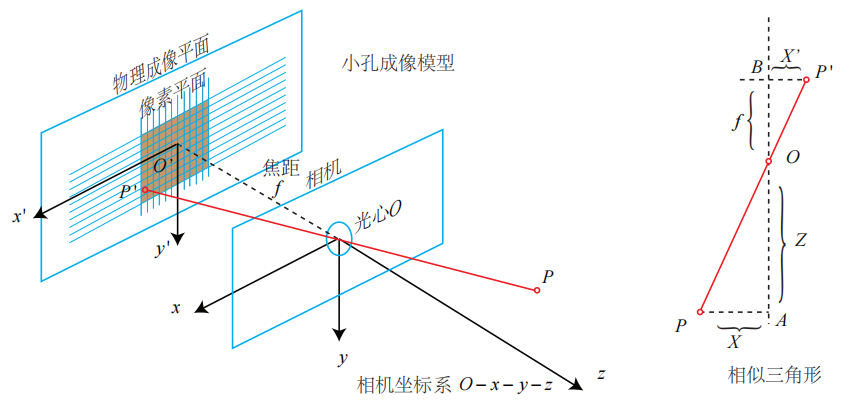
\includegraphics[width=14.5cm]{pinhole-camera}
	\caption{针孔相机成像原理图}
	\label{pinhole-camera}
\end{figure}

图\ref{pinhole-camera}解释了该模型的原理图,$O$是相机的光心,也是本算法中的虚拟视点,以$O$点为中心构建三维直角坐标系$O-x-y-z$,该坐标系成为相机坐标系,真实世界中的点$P$透过光心$O$落在光心后的物理成像平面$O'-x'-y'$上,该成像平面与$O-x-y$平面平行,投影点为$P'$,将光心$O$到成像平面的垂直距离记作焦距$f$,设$P$点坐标为$[X,Y,Z]^T$,$P'$坐标为$[X',Y',Z']^T$,则根据相似三角形的性质,有
\begin{equation}
	\label{eq: pinhole-camera}
	\frac{Z}{f}=-\frac{X}{X'}=-\frac{Y}{Y'}
\end{equation}
其中负号代表相机成像是道理的。为了实验与分析的方便,一般将成像平面至于相机前方,则\ref{eq: pinhole-camera}可变为
\begin{equation}
	\frac{Z}{f}=-\frac{X}{X'}=-\frac{Y}{Y'}
\end{equation}

整理得
\begin{equation}
	\label{eq: camera-to-plane}
	\left\{
	\begin{aligned}
		& X' = f\frac{X}{Z} \\
		& Y' = f\frac{Y}{Z}
	\end{aligned}
	\right.
\end{equation}

为了获得$P$点在图像中的像素,还需要做一次坐标转换,将成像平面坐标系转换为像素坐标系$o-u-v$。这两者之间相差一个尺度和位移变换,,假设$P$点的像素坐标为$[u,v]^T$,则其数学表达式为
\begin{equation}
	\label{eq: pinhole-tranform}
	\left\{
	\begin{aligned}
		& u = \alpha X'+ c_x\\
		& v = \beta Y' + c_y
	\end{aligned}
	\right.
\end{equation}
其中$\alpha, \beta$表示$u$轴和$v$轴上的缩放系数,$c_x, c_y$代表成像中心在像素坐标系下的坐标。将式\ref{eq: camera-to-plane}带入上式,并写成矩阵的形式可得
\begin{equation}
	\label{eq: world-to-camera}
	Z\begin{pmatrix}u\\v\\1\end{pmatrix}=
	\begin{pmatrix}
		f_x & 0 & c_x\\
		0 & f_y & c_y\\
		0 & 0 & 1
	\end{pmatrix}
	\begin{pmatrix}X\\Y\\Z\end{pmatrix}
	\triangleq \boldsymbol{KP}
\end{equation}
其中$\boldsymbol{P}$是真实世界的像素坐标,$\boldsymbol{K}$定义为相机的内参矩阵。

通常来讲,按照\ref{eq: world-to-camera}计算出来的$u, v$值往往是小数,因此可以采用插值法对每个点的RGB通道进行插补,常用的插值方法有最近邻插补法、基于三角形的线性插补法、以及基于三角形的三次插补法。这几种方法的效果依次递增,但同样计算开销也较大。同时需要注意的是,通过后两种方法得到的颜色通道值有可能超出0-255的范围,因此需要进行截断。

\subsection{实验结果}
本章利用表\ref{blk360-data}中测站4的数据进行了实验,图像生成算法的原理示意图如图\ref{camera-tsinghua}所示。
\begin{figure}
	\centering
	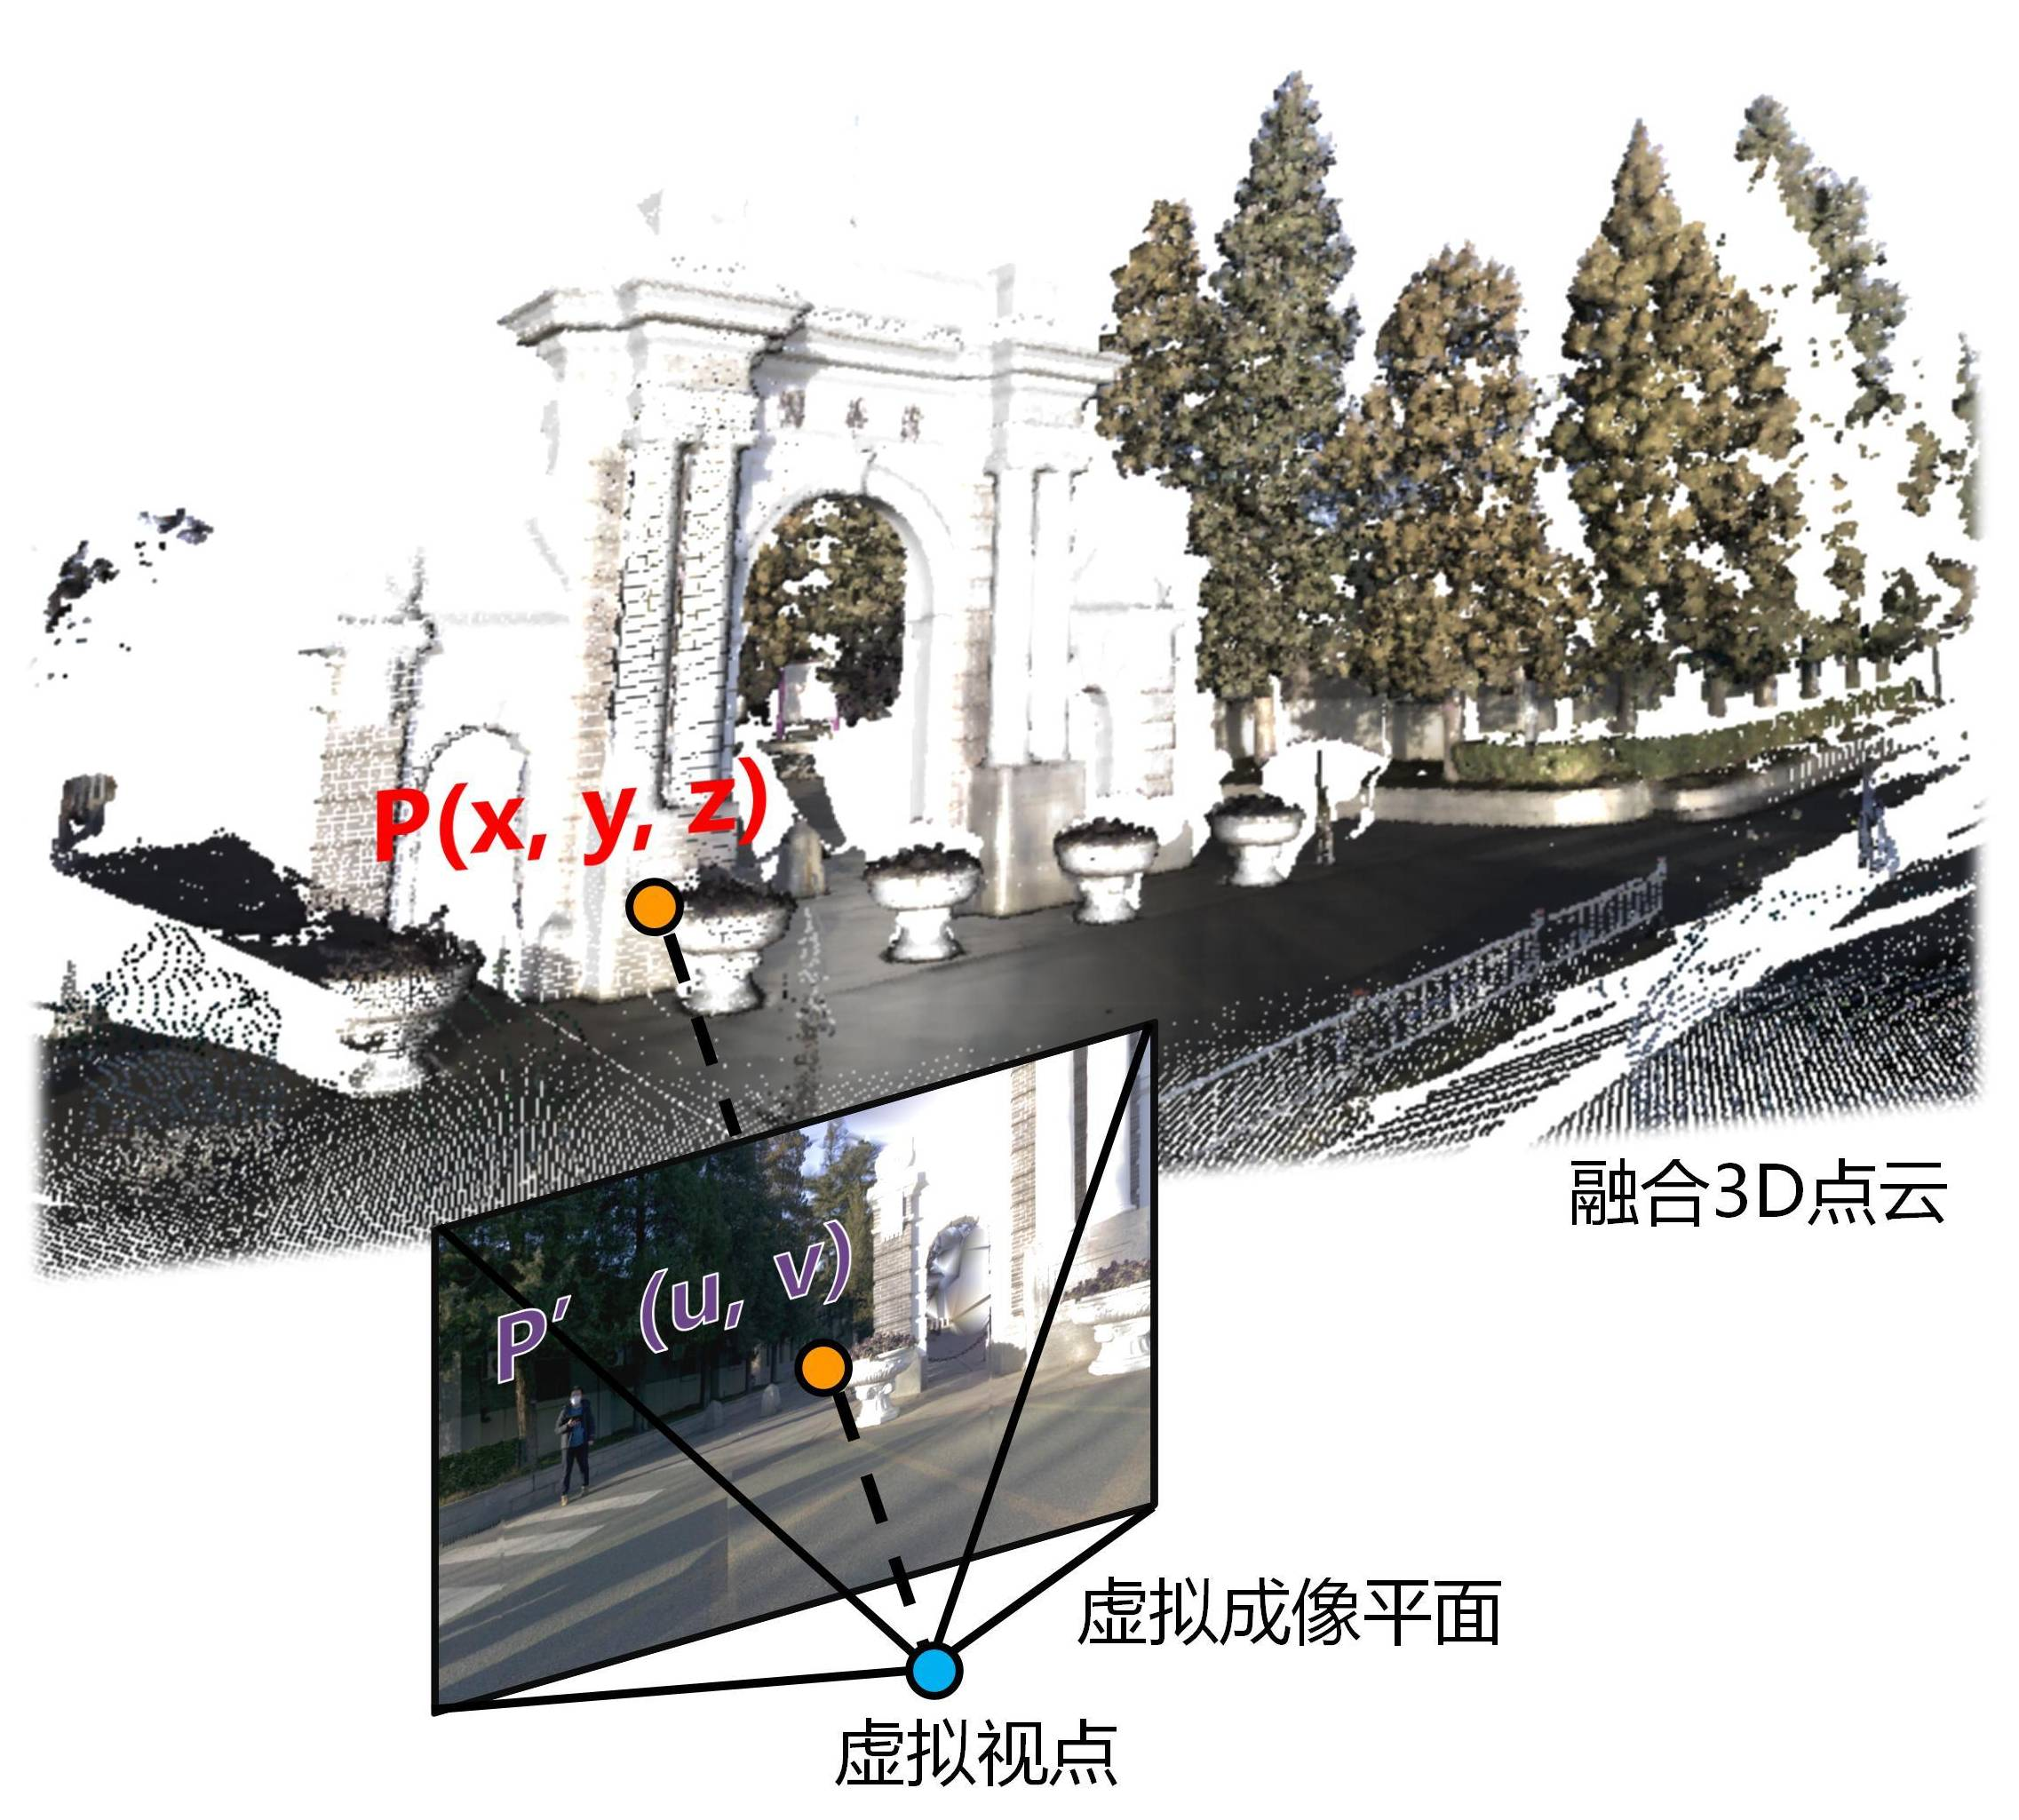
\includegraphics[width=10cm]{camera-tsinghua.jpg}
	\caption{虚拟成像原理图}
	\label{camera-tsinghua}
\end{figure}

设置虚拟相机的焦距$f=1$,成像平面为$z=1$的平面,同时为了固定成像平面大小,将水平视角设为$90^\circ$,垂直视角设为$60^\circ$,图像大小$960\times640$,$x,y,z$轴的轴旋转角$p,t,r$分别为$-90^\circ,90^\circ,0^\circ$,采用线性插值的方法对像素点插值,结果如图\ref{gate-from-pc-linear}所示。由于这里采用了室外点云进行实验,部分区域(如天空)存在大面积点缺失现象,直接采用插值的结果会与真实成像结果差距较大,因此为了避免失真,在算法最后对所得到的图像进行掩模处理,将大面积无投影的区域颜色置为纯黑色。
\begin{figure}
	\centering
	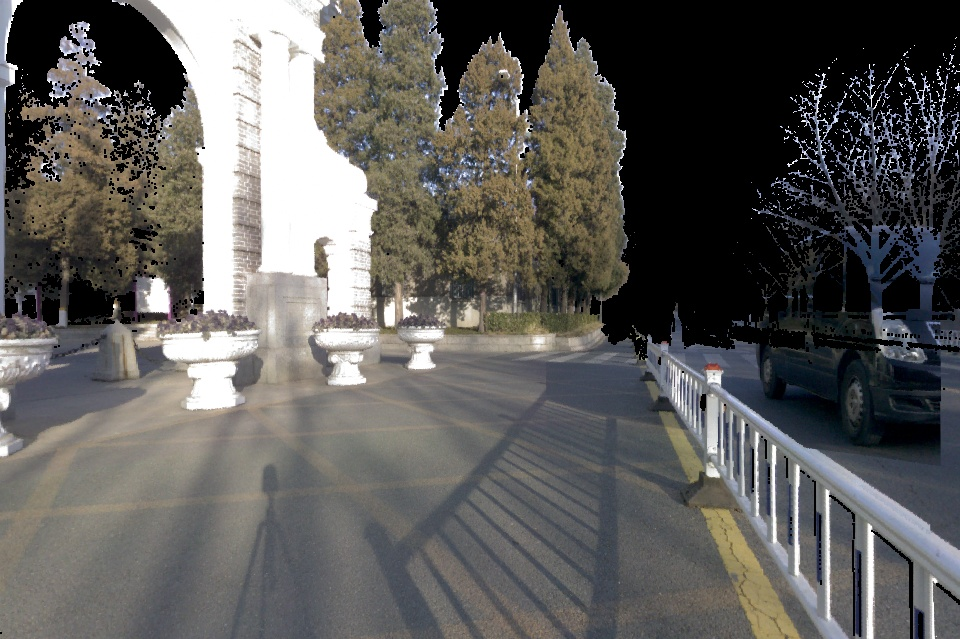
\includegraphics[width=12cm]{gate-from-pc-linear}
	\caption{点云-平面映射实验结果}
	\label{gate-from-pc-linear}
\end{figure}

从图中中可以得到,从点云中恢复的平面图像能够较好的模拟真实相机的拍摄效果,这可以为下一步图像之间的匹配提供了较好的输入。

\section{全景畸变校正}
由于全景相机能够带来更广阔的视野,为后续特征匹配寻找关键点提供更多信息,因此在本研究中采用全景相机进行定位,但全景相机由于其自身的成像原理,会带来很大的畸变,因此在本节中主要介绍这种相机的成像原理,并对其进行畸变校正。
\subsection{全景成像原理}
与图\ref{pinhole-camera}所示的针孔相机不同,全景相机的投影面不是一个平面,而是一个球面,如图\ref{equiretangular}所示,首先建立相机坐标系$O-x-y-z$,在相机坐标系下,全景相机将真实世界中的一点$\boldsymbol{P}^w=(x^w, y^w, z^w)$投影到单位球上$\boldsymbol{P}^c=(x^c,y^c,z^c)$,即满足$\|\boldsymbol{P}^c\|=1$,根据相似三角形,有
\begin{equation}
	\dfrac{x^w}{x^c} = \dfrac{y^w}{y^c} = \dfrac{z^w}{z^c}
\end{equation}

转换为球坐标系,有
\begin{equation}
	\left\{
	\begin{aligned}
		&r = \sqrt{(x^c)^2+(y^c)^2+(z^c)^2}\\
		&\theta = \arccos \dfrac{z^c}{r}\\
		&\varphi = \arctan \dfrac{y^c}{x^c}
	\end{aligned}
	\right.
\end{equation}

同样,从相机坐标系转换到像素坐标系需要进行尺度和平移变换,其变换形式与式\ref{eq: pinhole-tranform}类似,如下
\begin{equation}
	\left\{
	\begin{aligned}
		& u = \alpha \theta+ c_x\\
		& v = \beta \varphi + c_y
	\end{aligned}
	\right.
\end{equation}

\begin{figure}
	\centering
	\subcaptionbox{相机坐标系\label{equiretangular}}	{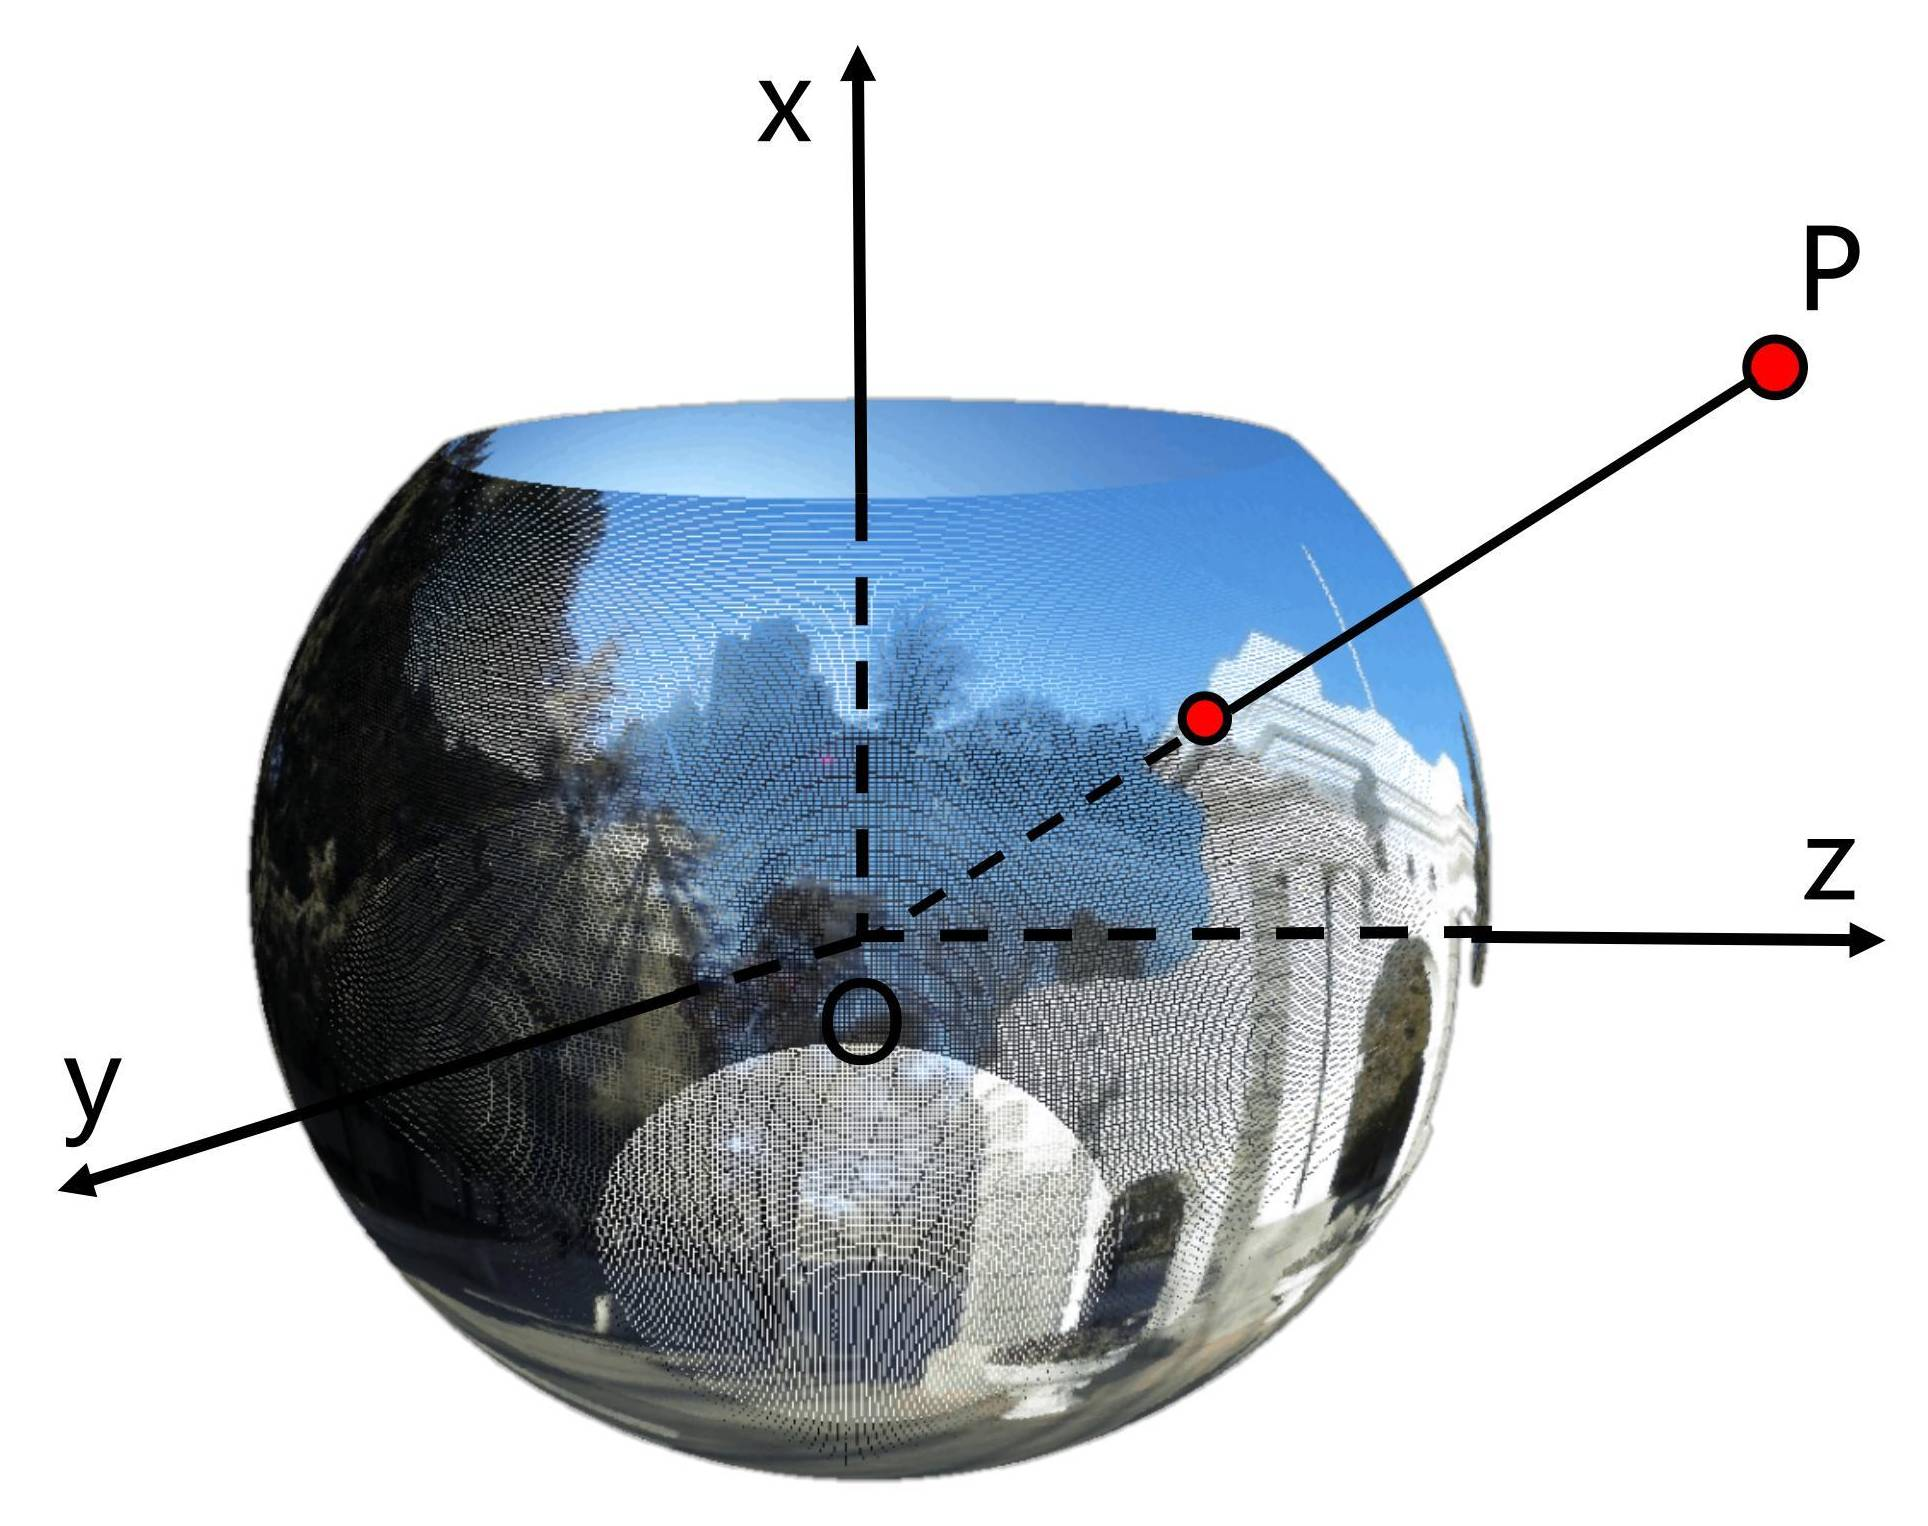
\includegraphics[width=7cm]{equiretangular}}
	\subcaptionbox{球坐标系\label{sph-coordinate}}
	{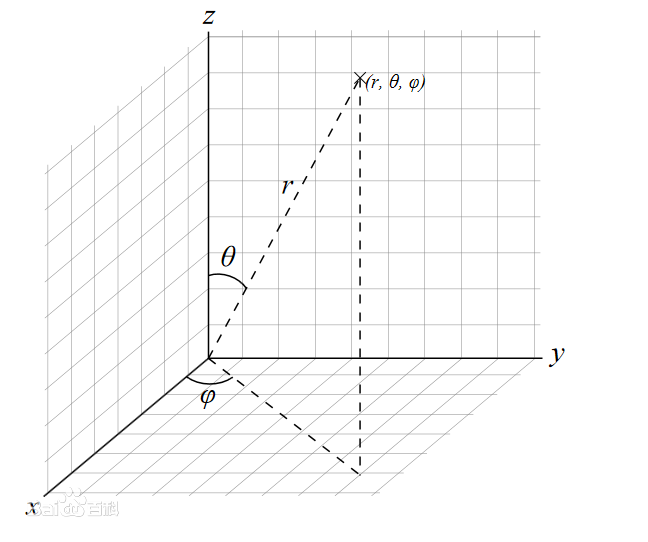
\includegraphics[width=7cm]{sph-coordinate}}
	\caption{全景相机成像原理图}
	\label{omnidirectional-camera}
\end{figure}

\subsection{畸变校正原理}
如图\ref{camera-distortion}所示,在照片成像的过程中,由于相机本身的构造或者人为组装上的偏差,相机成像后往往会带来畸变,造成空间上的直线投影到成像平面后产生了弯曲,在知道畸变参数之后,往往可以对畸变图像进行校正恢复。
\begin{figure}
	\centering
	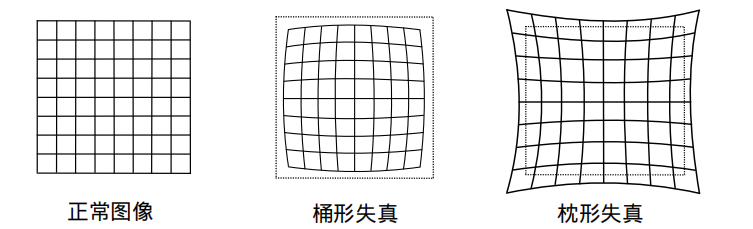
\includegraphics[width=14cm]{camera-distortion}
	\caption{相机畸变示意图}
	\label{camera-distortion}
\end{figure}

与针孔相机带来的畸变不同的是,全景相机的畸变是本身成像平面的弯曲带来的,因此可以利用上一节中介绍的原理,对全景相机图像进行畸变校正,根据弯曲方向的不同可以将畸变分为桶形失真和枕形失真两类。

如图\ref{pano-to-plane-theory}所示,该算法使用了一个新的成像平面$z=1$,并确定了平面图像的大小$H\times W$,因此类似于在点云中的虚拟成像原理(见第\ref{point-cloud-to-plane}节),可以将全景图的每个像素看做三维空间中单位球上的若干个点,从$O$点出发连接这些点的射线与$z=1$平面的交点即为平面图投影点,同样这些点在新成像平面上的坐标值大多是小数,因此最后需要通过插值法得到某一视角下的畸变校正结果。
\begin{figure}
	\centering
	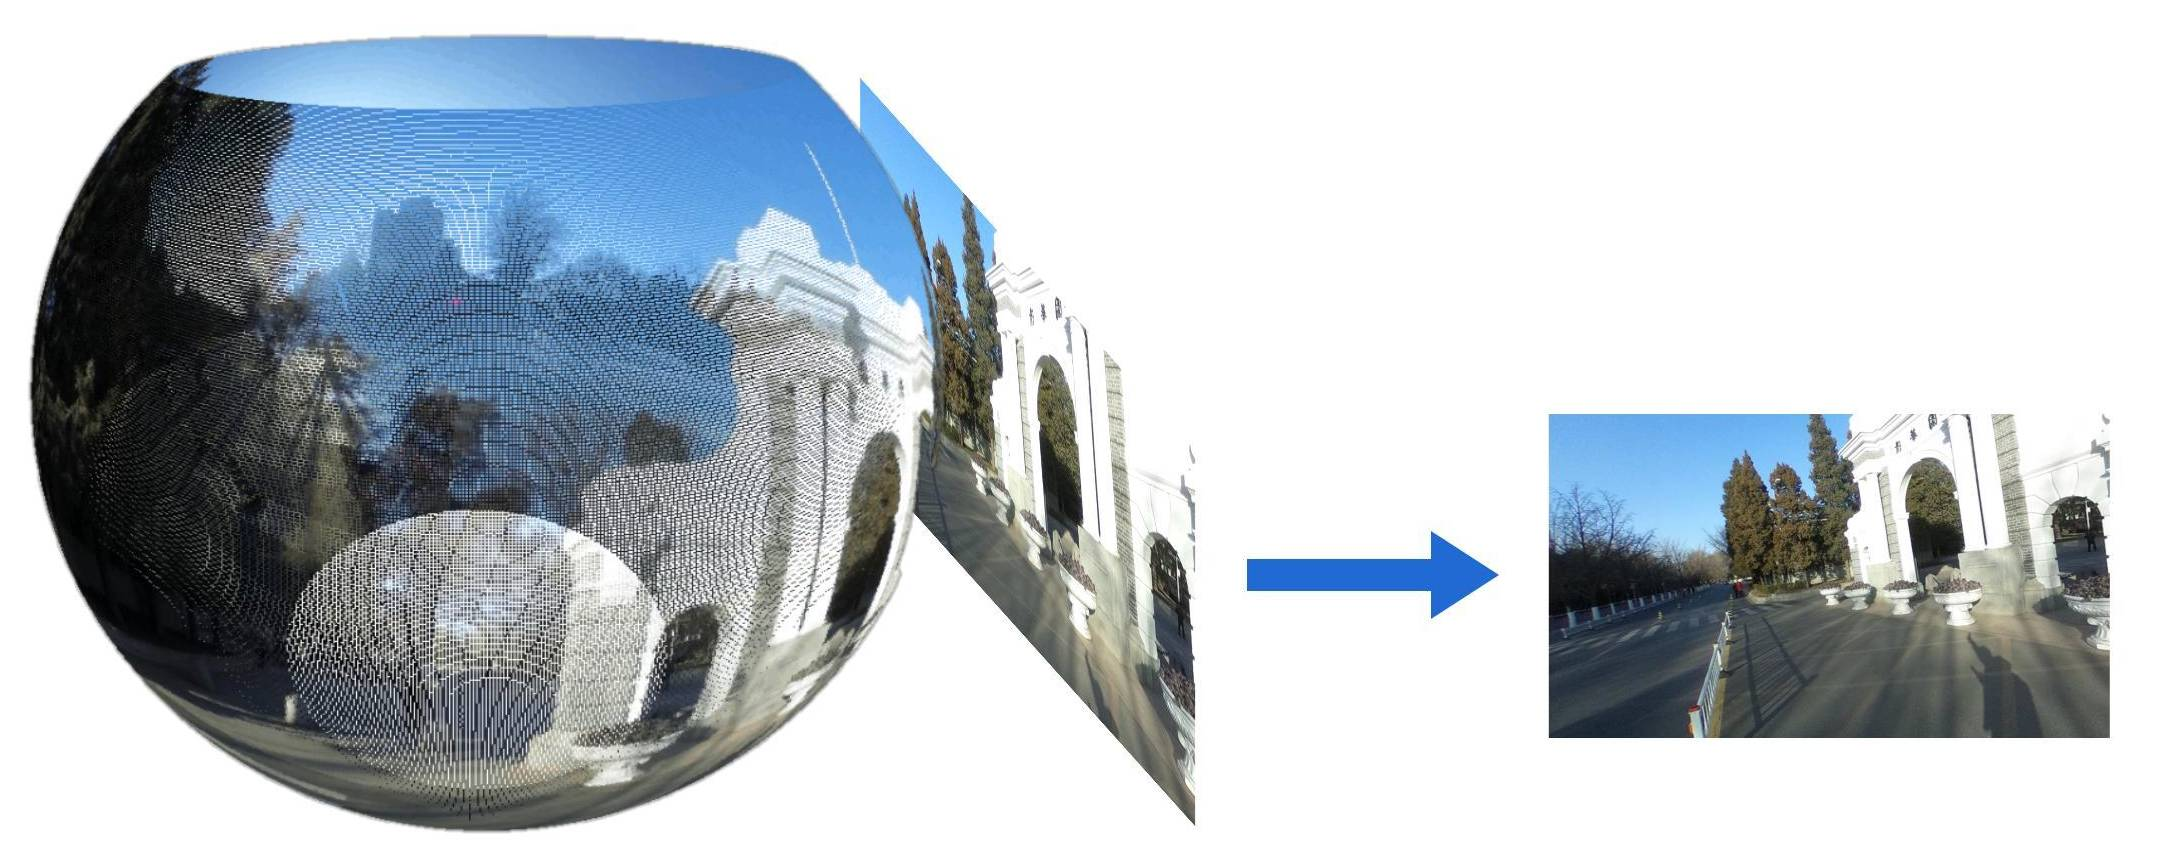
\includegraphics[width=14cm]{pano-to-plane-theory}
	\caption{全景图像畸变校正示意图}
	\label{pano-to-plane-theory}
\end{figure}

\subsection{实验结果}
本节实验选择理光全景相机RICHO THETA V作为拍摄设备,如图\ref{richo}所示,该设备通过前后两个鱼眼镜头拍摄的图像来合成全景图,拥有ISO3200的图像感光度和6400的视频感光度,以及1/2500秒的快门速度,并且支持4K 60fps高清视频录制。
\begin{figure}
	\centering
	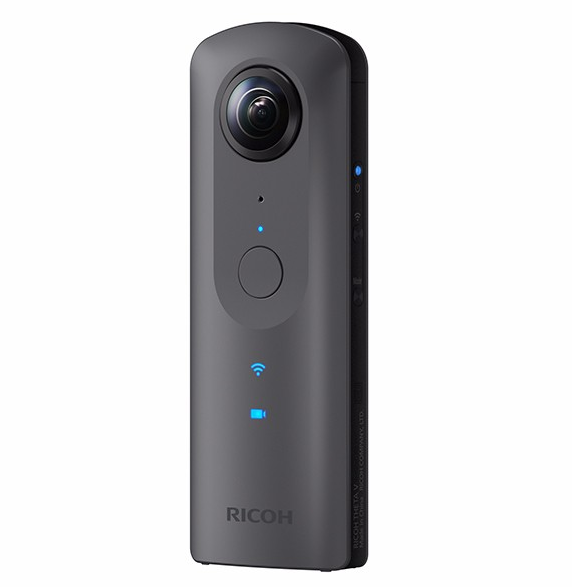
\includegraphics[width=6.5cm]{richo}
	\caption{RICHO THETA V全景相机}
	\label{richo}
\end{figure}

使用该设备在二校门处拍摄一张全景图像,如图\ref{gate-pano},相机拍摄的全景视图固定水平视角为$90^\circ$,垂直视角为$60^\circ$,分别在水平转向角为$45^\circ, 135^\circ, 225^\circ, 315^\circ$的位置生成校正图,其结果如图\ref{pano-to-plane-result}所示。
\begin{figure}
	\centering
	\subcaptionbox{二校门全景图像\label{gate-pano}}	{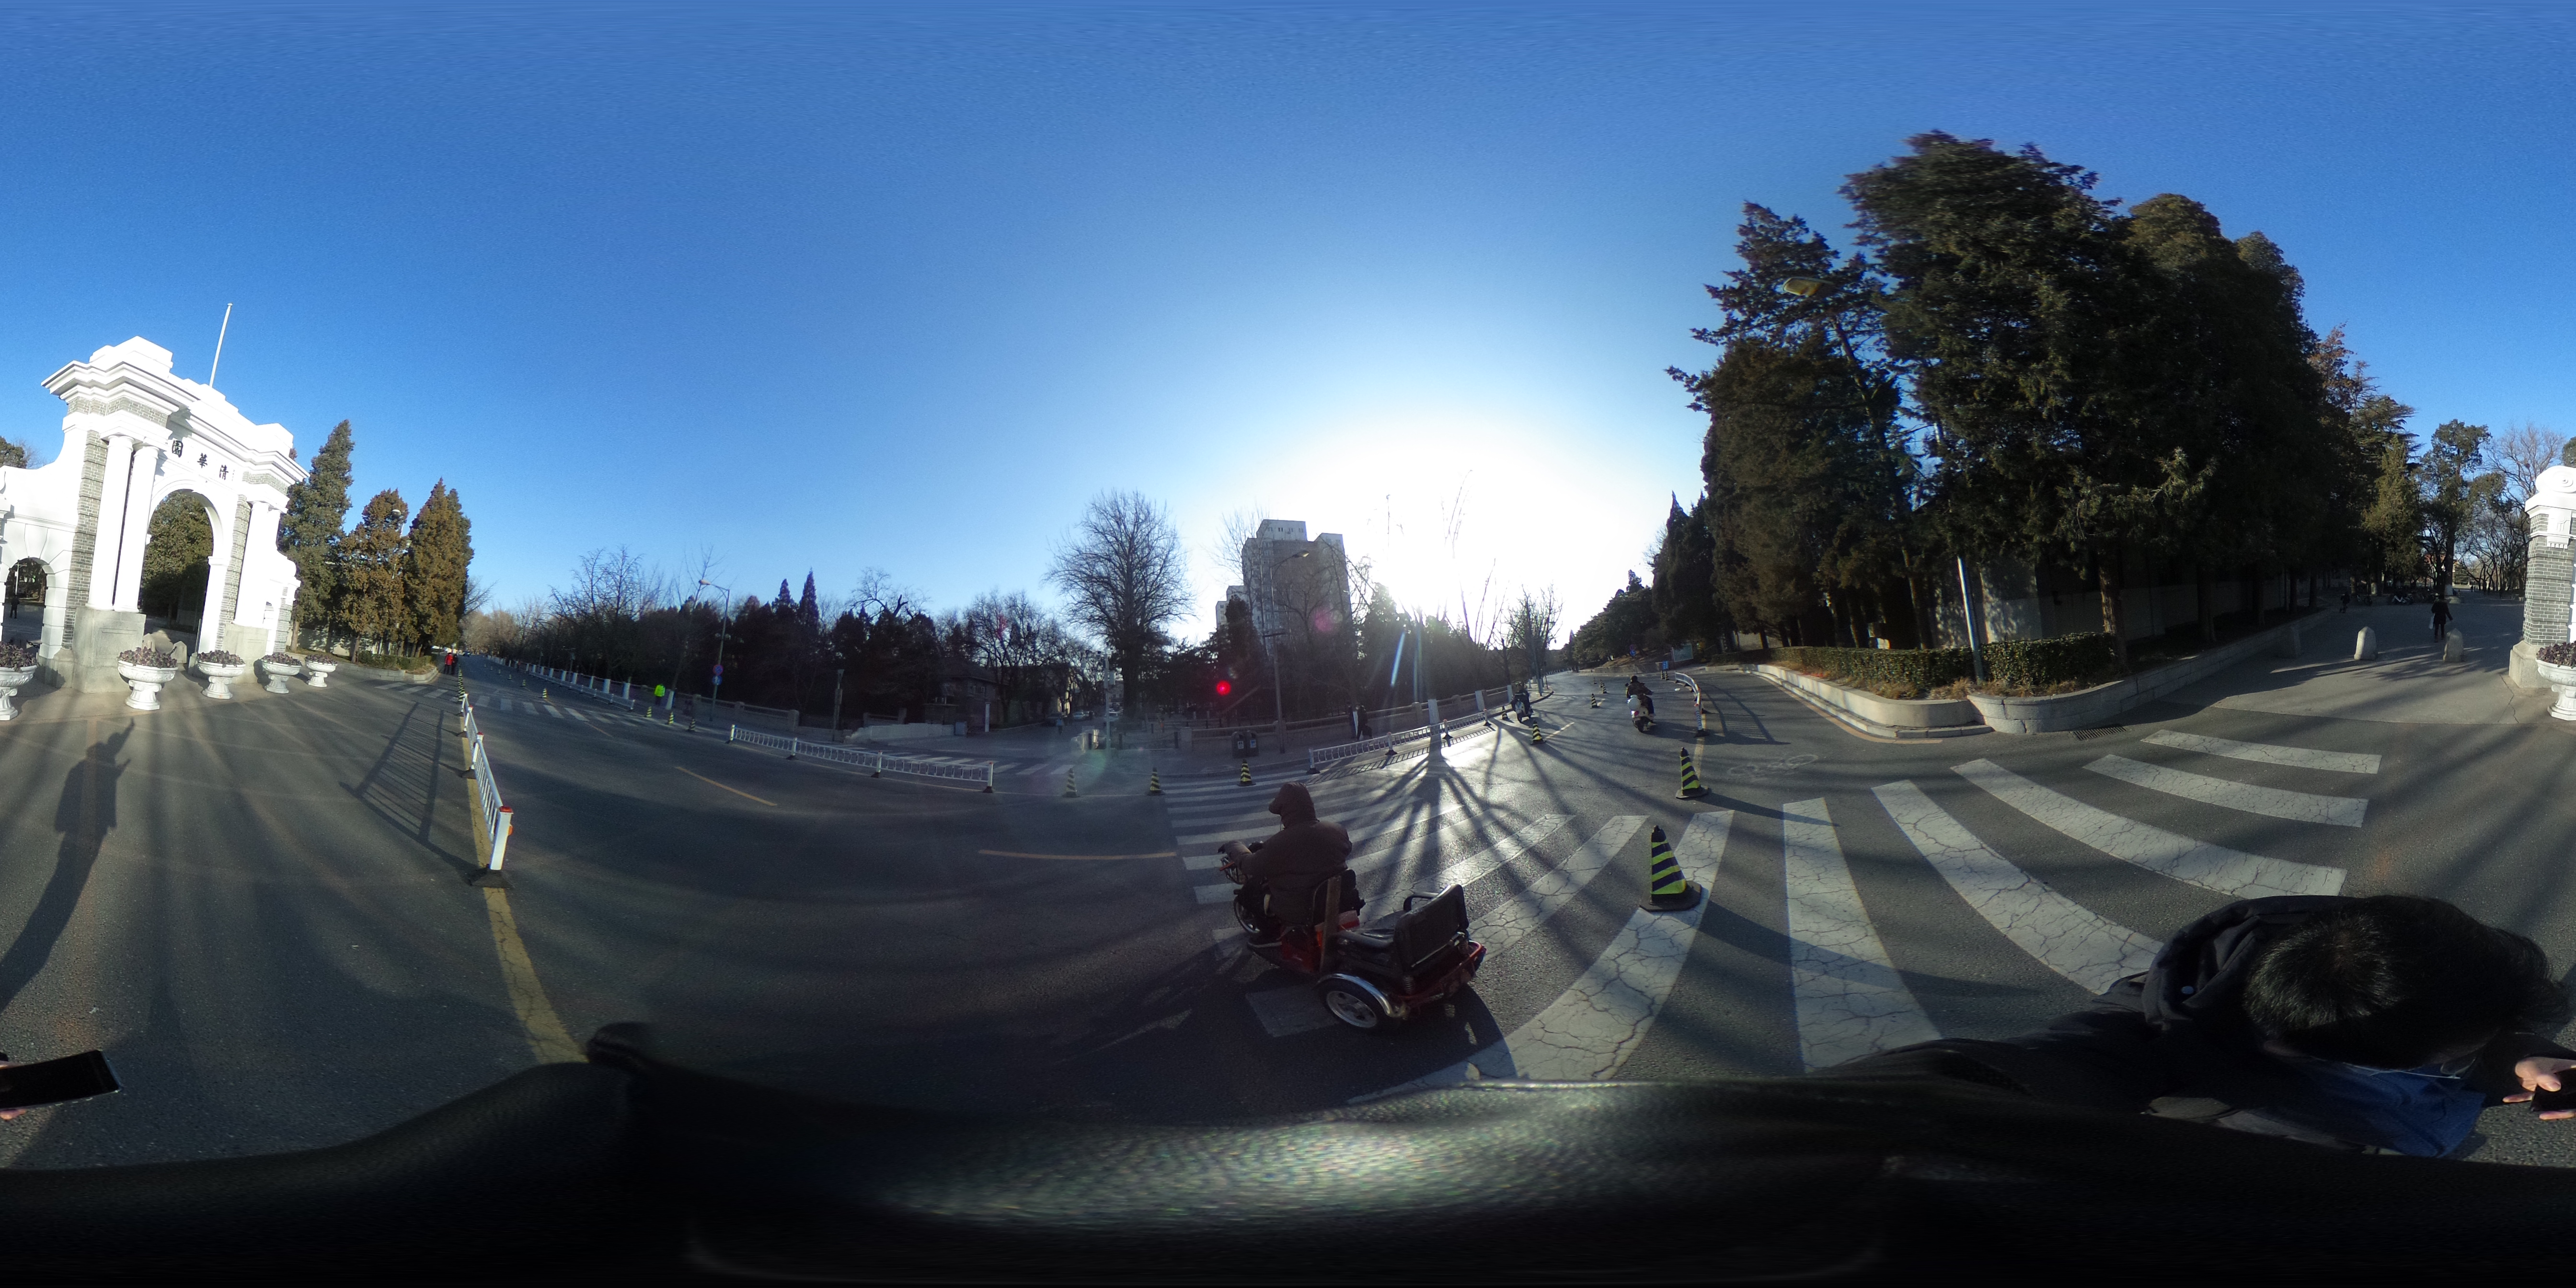
\includegraphics[width=10cm]{gate-pano}}\\
	\subcaptionbox{局部畸变校正结果\label{pano-to-plane-result}}
	{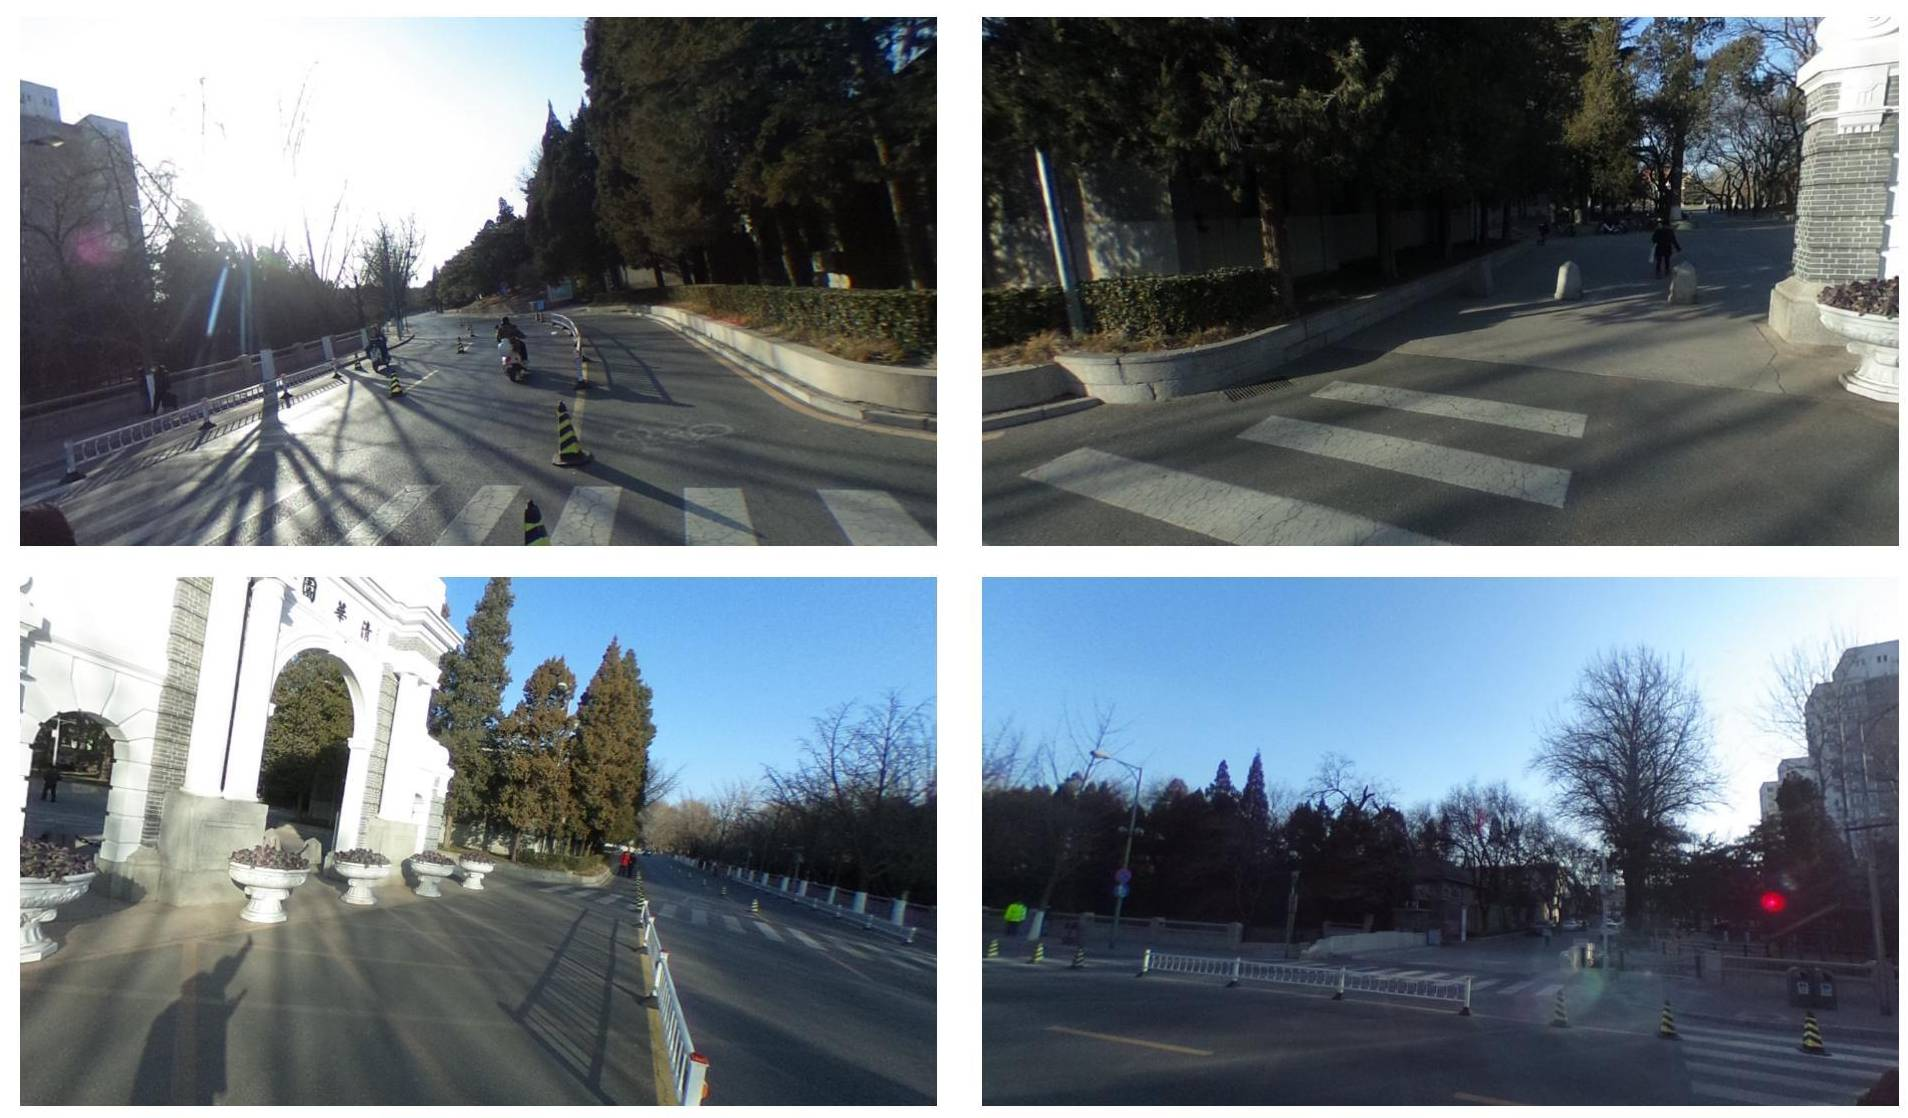
\includegraphics[width=13cm]{pano-to-plane-result}}
	\caption{全景畸变校正实验数据及结果}
	\label{pano2plane-data-result}
\end{figure}

\section{基于SOSNet的图像特征提取与匹配}
本章先通过点云合成的2D图像与全景图的2D图像之间进行特征点的匹配,然后进行相机位姿的估计。这一方法的主要问题是通过点云生成的视图与定位时的视图可能在光照条件、位置等方面存在着较大的变换,因此需要一个鲁棒的图像特征提取与匹配算法。

本文采用了SOSNet的方法,该网络将二阶相似性(Second Order Similarity)纳入损失函数当中,在多个基准数据集上收获了较好的性能。
\subsection{网络结构及损失函数}
该网络的结构与L2-Net\cite{tian2017l2}相同,如图\ref{l2net}所示,它采用了一个全卷积的结构,降采样通过一个stride为2的卷积层实现。在每层卷积层之后连接了BN层,最后将局部响应归一化层(LRN)\cite{krizhevsky2012imagenet}作为输出层来生成描述符。该网络能够将输入的$32\times 32$的patch映射为128维的向量。
\begin{figure}
	\centering
	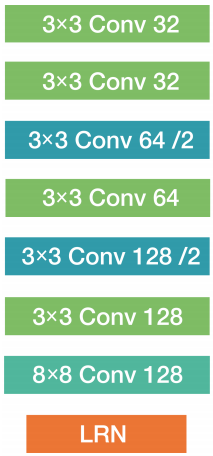
\includegraphics[width=3.5cm]{l2net}
	\caption{L2-Net网络结构}
	\label{l2net}
\end{figure}

与L2-Net不同的是,SOS-Net在训练时的损失函数设计,不仅仅考虑了特征之间的一阶相似度(FOS),也将二阶相似度(SOS)纳入其中,其中一阶相似度的计算如下
\begin{equation}
	\mathcal{L}_{FOS}=\frac{1}{N}\sum_{i=1}^N \max\left(0, t+d_i^{\text{pos}}-d_i^{\text{neg}}\right)^2
\end{equation}
其中
\begin{equation}
	d_i^{\text{pos}} = d\left(\boldsymbol{x}_i, \boldsymbol{x}_i^+\right)
\end{equation}
\begin{equation}
	d_i^{\text{neg}} = \min_{\forall j, j\neq i}\left(d(\boldsymbol{x}_i, \boldsymbol{x}_j), d(\boldsymbol{x}_i, \boldsymbol{x}_j^+), d(\boldsymbol{x}_i^+, \boldsymbol{x}_j),
	d(\boldsymbol{x}_i^+, \boldsymbol{x}_j^+)\right)
\end{equation}
式中$\boldsymbol{x}_i$和$\boldsymbol{x}_i^+$分别表示两幅图像中匹配的patch特征,$d_i^{\text{pos}}$衡量了正确的匹配对之间的欧氏距离,$d_i^{\text{neg}}$表示了匹配对之间的距离。

对于两个匹配对$\boldsymbol{x}_i$和$\boldsymbol{x}_i^+$,首先定义两者的二阶相似性
\begin{equation}
	d^{(2)}(\boldsymbol{x}_i, \boldsymbol{x}_i^+) = \sqrt{\sum_{j\neq i}^{N}\left(d(\boldsymbol{x}_i, \boldsymbol{x}_j), d(\boldsymbol{x}_i^+, \boldsymbol{x}_j^+)\right)^2}
\end{equation}

基于SOS的正则项可以表示为所有patch与对应patch的二阶相似性平均值
\begin{equation}
	\mathcal{R}_{SOS}=\frac{1}{N}\sum_{i=1}^{N}d^{(2)}\left(\boldsymbol{x}_i,\boldsymbol{x}_i^+\right)
\end{equation}

总loss看做一阶相似性和二阶相似性的直接加和
\begin{equation}
	\mathcal{L}_T=\mathcal{L}_{FOS}+\mathcal{R}_{SOS}
\end{equation}

\subsection{特征提取与匹配结果}
本实验分别从点云生成的平面图和通过全景相机生成的局部平面图中各选择一帧,首先用BRISK算法\cite{leutenegger2011brisk}对特征点进行提取,该算法能够保证特征提取的旋转不变性和尺度不变性,特征点提取结果如图\ref{brisk-feature-extract},上半部分为点云生成的图像,下半部分为利用全景相机生成的图像,其中前者提取到的特征点数为231个,后者提取的特征点数为230个。
\begin{figure}
	\centering
	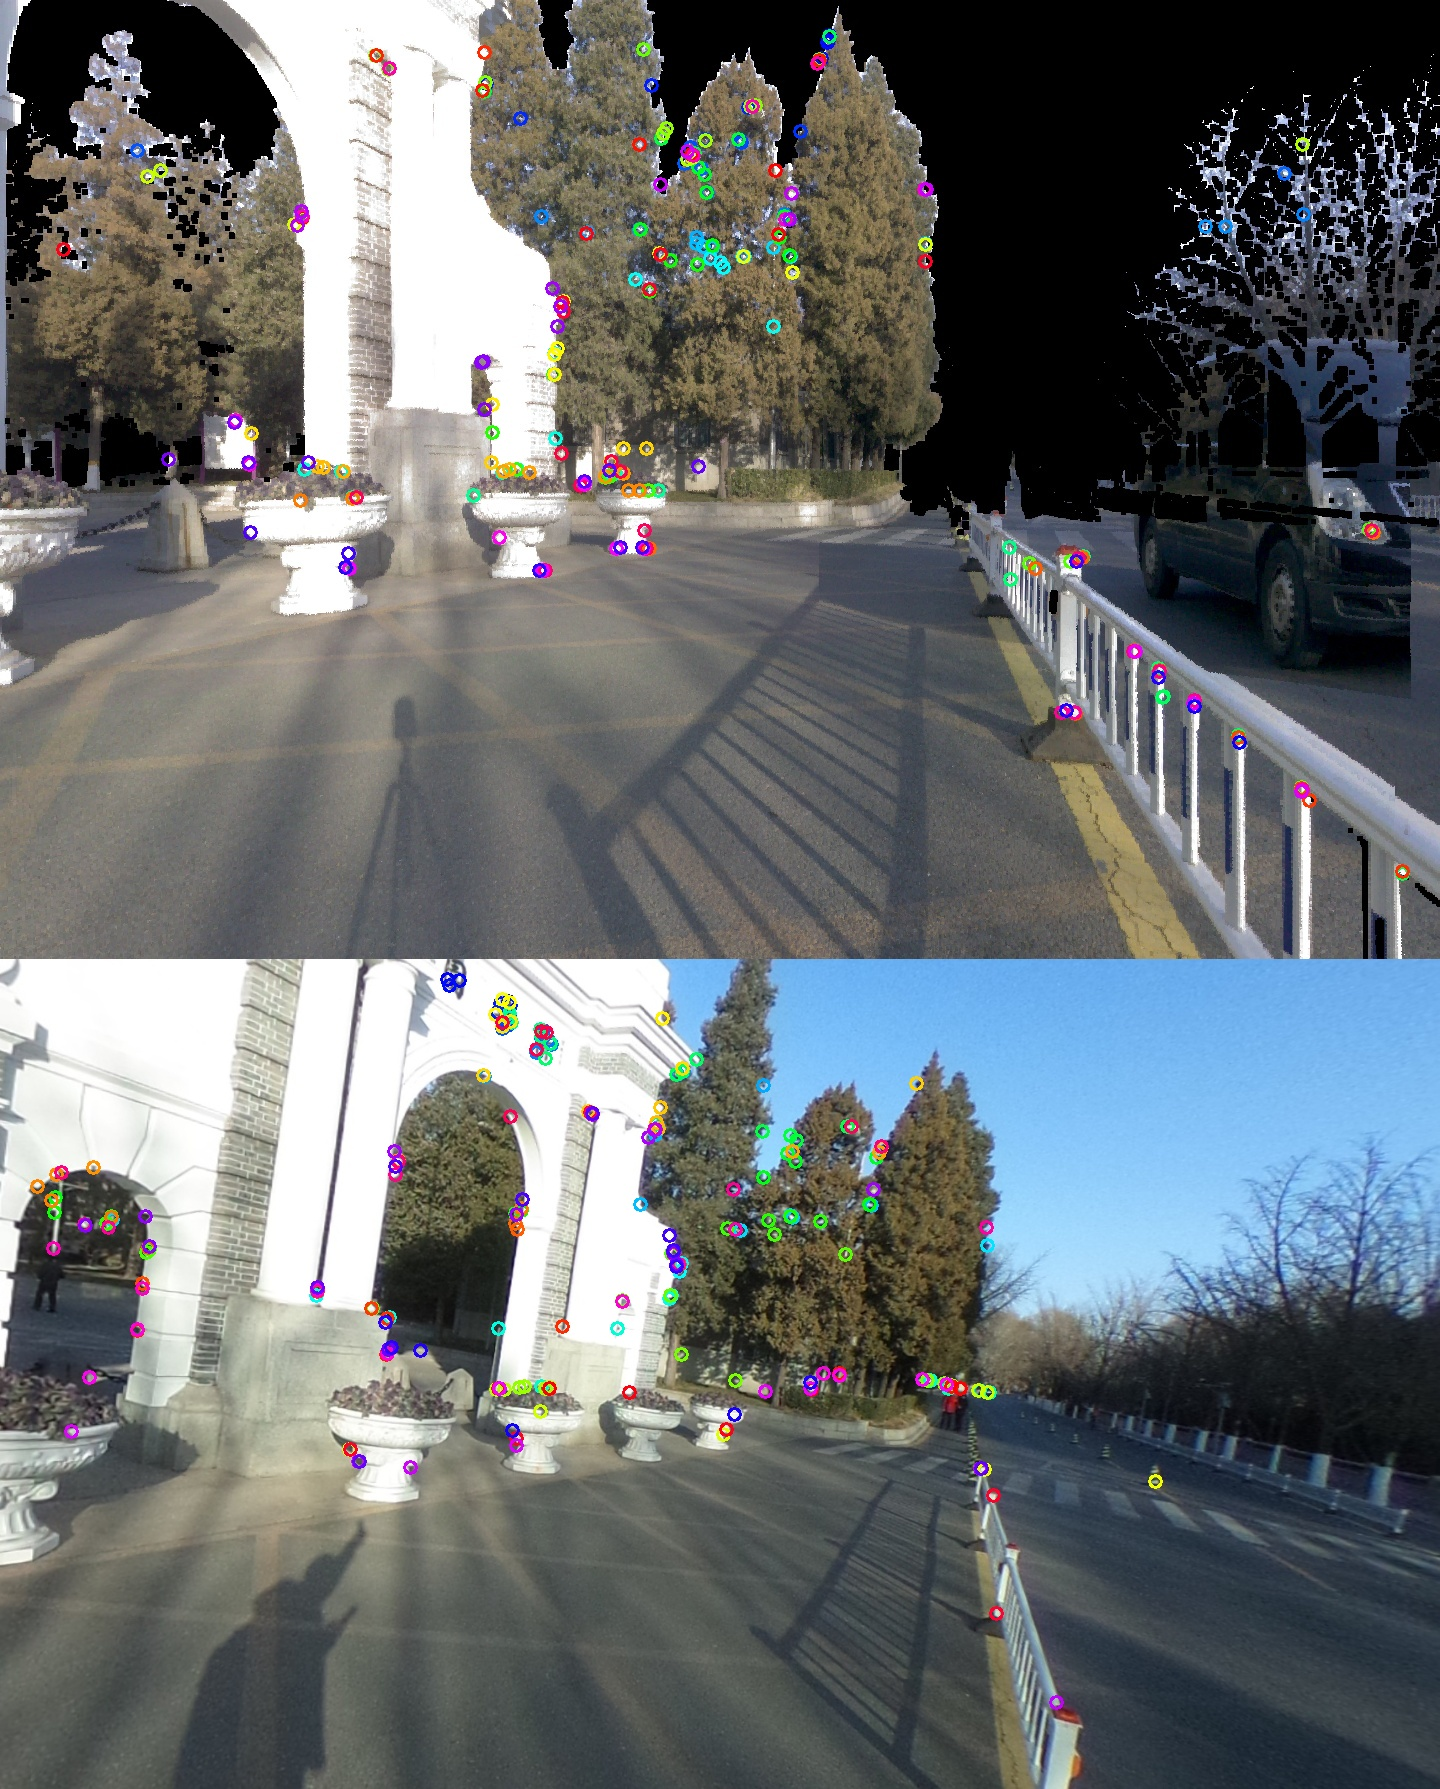
\includegraphics[width=8cm]{brisk-feature-extract}
	\caption{BRISK算法特征点提取}
	\label{brisk-feature-extract}
\end{figure}

在特征提取算法中,首先通过SOSNet生成两张图片中每个特征点的特征描述符,对于每个查询点$\boldsymbol{x}_q$,寻找其在另一张图中的前2个最佳匹配结果$\boldsymbol{x}_1, \boldsymbol{x}_2$,若$\|\boldsymbol{x}_q - \boldsymbol{x}_1\|<0.88\|\boldsymbol{x}_q - \boldsymbol{x}_2\|$,则该匹配被认为是好的匹配,$\boldsymbol{x}_q$和$\boldsymbol{x}_1$被标记为匹配点。

利用上述算法对二校门的两张图片之间的特征进行匹配,其结果如图\ref{sosnet-match-result},为了对比该算法的效果,本文同时采用了ORB算法进行了特征匹配,其结果如图\ref{orb-match-result}。可见,利用SOSNet网络能够得到14对特征匹配对,且匹配基本正确;而使用ORB算法虽然得到了21对特征匹配对,但基本均为误匹配,效果不如SOSNet。
\begin{figure}
	\centering
	\subcaptionbox{SOSNet特征匹配结果\label{sosnet-match-result}}	{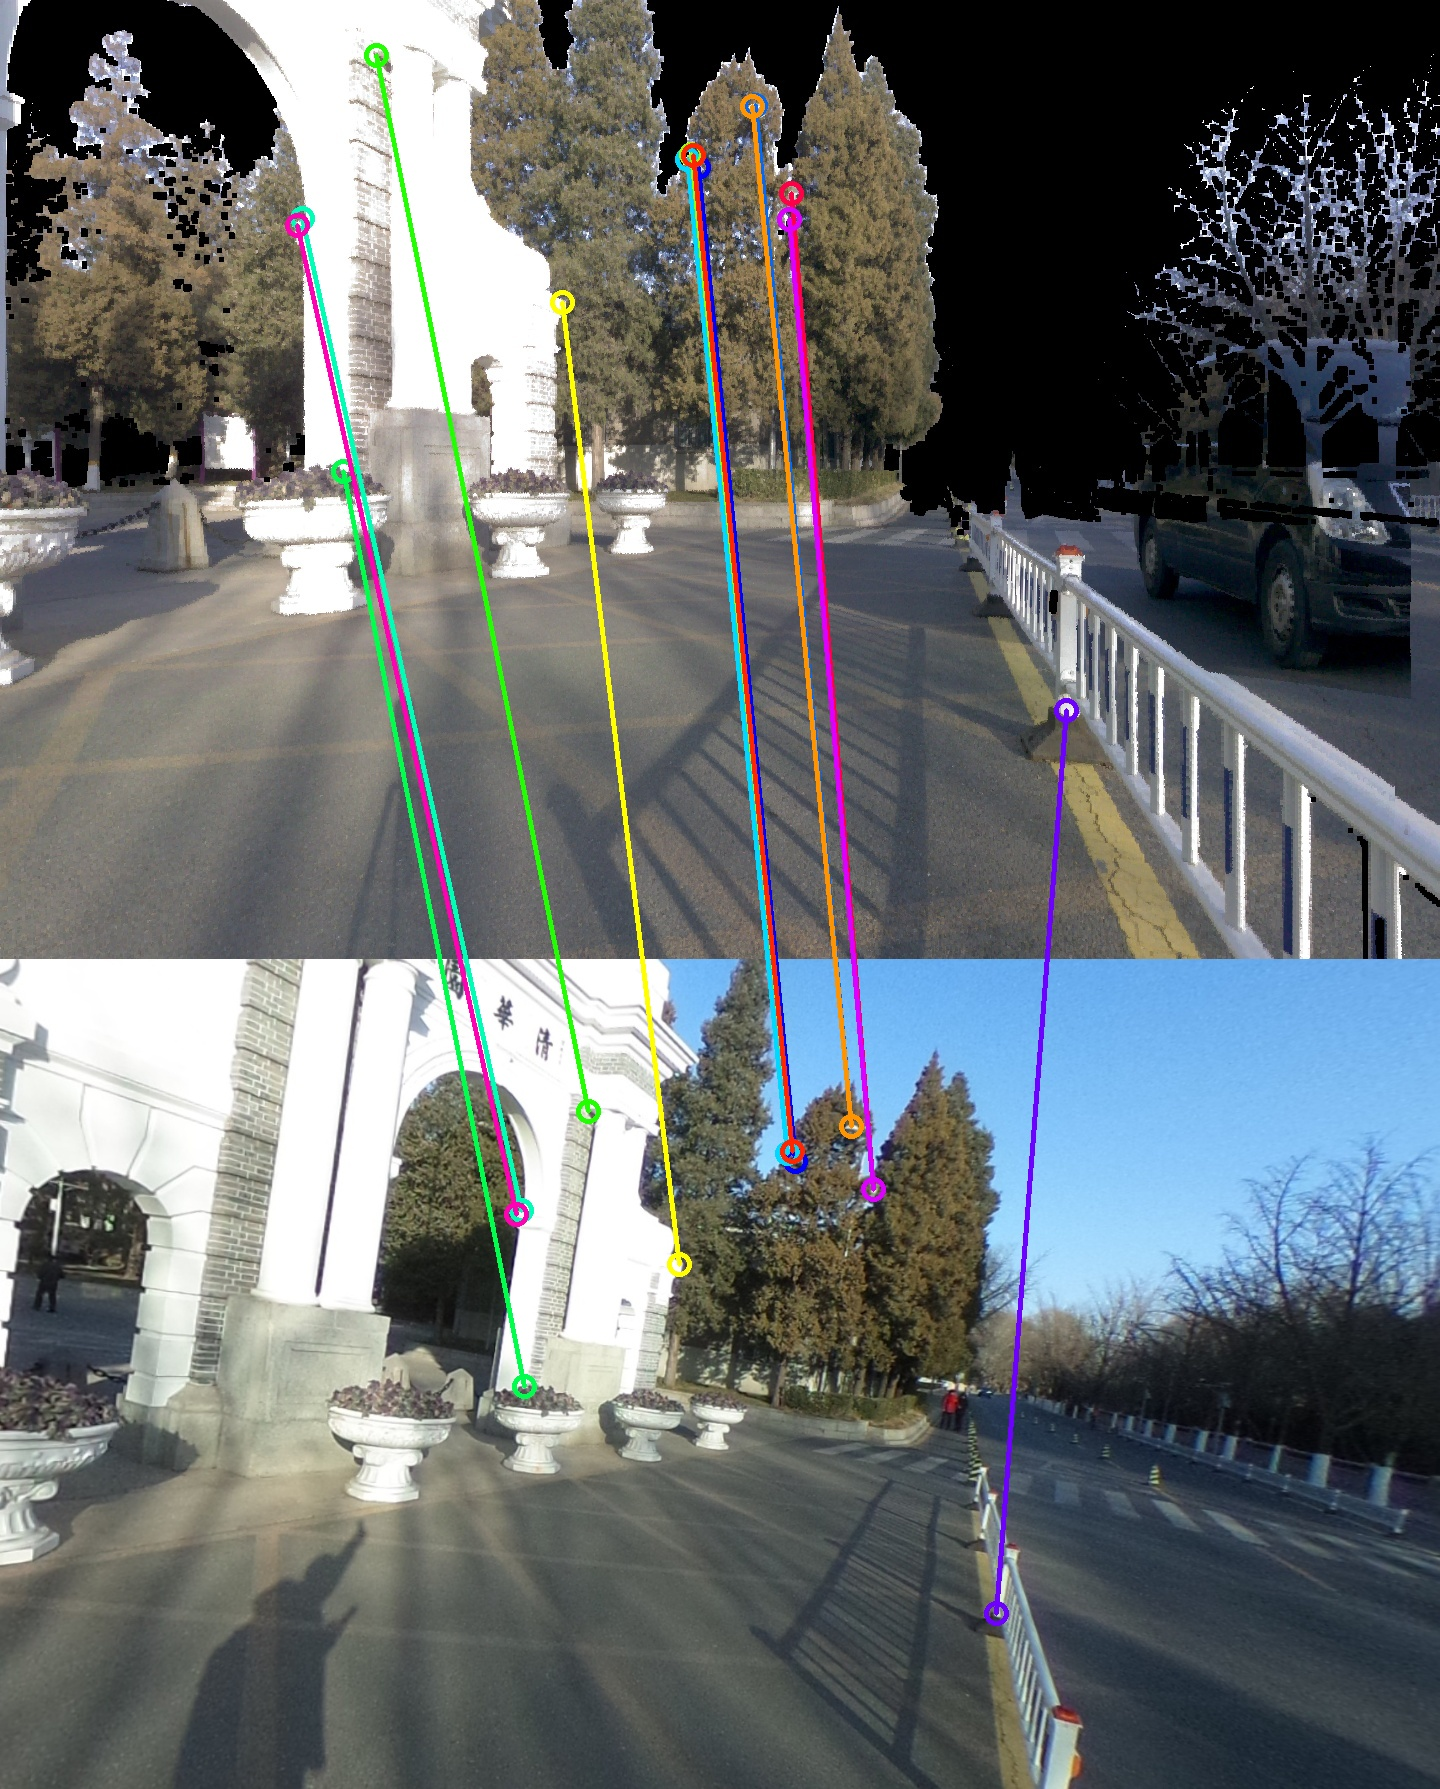
\includegraphics[width=7cm]{sosnet-match-result}}
	\subcaptionbox{ORB算法特征匹配结果\label{orb-match-result}}
	{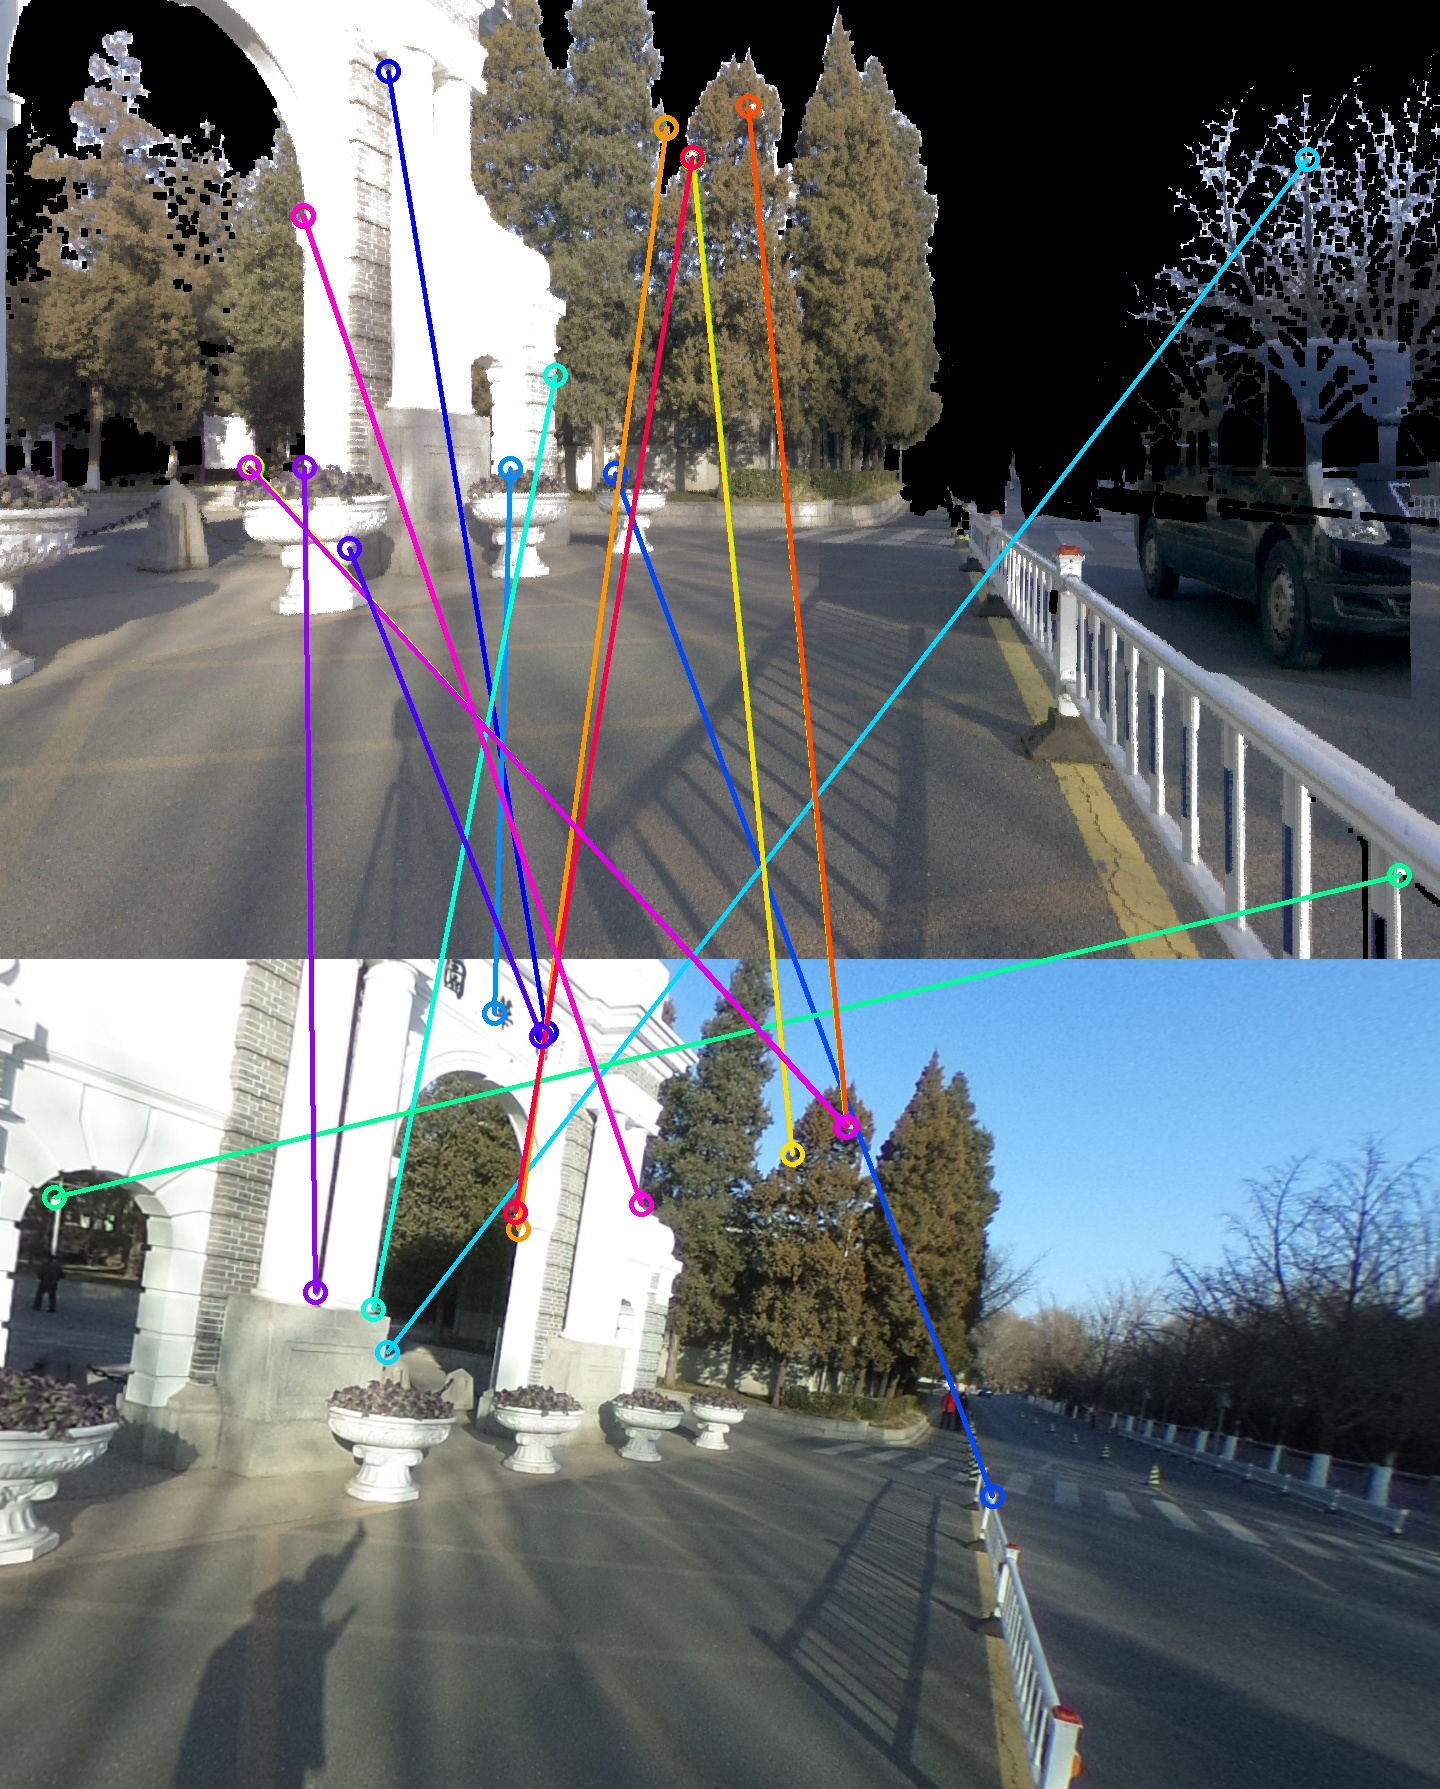
\includegraphics[width=7cm]{orb-match-result}}
	\caption{特征匹配结果及对比}
	\label{match-result}
\end{figure}

传统方法与基于学习的方法之所以在本研究中的特征提取任务上表现差异较大,主要是因为利用点云投影算法得到的平面图,与真实图像之间有所差距,同时两帧图像的位置差别也较大,因此常规的特征提取算法往往难以产生好的效果,而使用深度学习方法能够鲁棒地提取特征描述子,同时得益于图像二阶相似性在训练中的应用,使得相同匹配patch的特征描述符在欧式空间较为接近,因此产生了更好的匹配效果。

\section{基于对极约束的定位算法}
\subsection{对极约束}
在三维空间中,同一个点在两个不同相机的成像平面上的投影位置与这两个相机之间的运动和它们的内参之间存在着一个关系,这种关系被称为对极约束,因此,利用若干点对的对应关系,就能求取两个相机之间的运动。在上一节中,本文利用了SOSNet,对在点云某一位置生成的图像和全景相机图像之间的特征点进行了鲁棒的匹配,因此可以将点云的位置看做参考坐标系,利用对极约束求取这两者之间的运动,从而得到全景相机在点云中的相对位置。

\begin{figure}
	\centering
	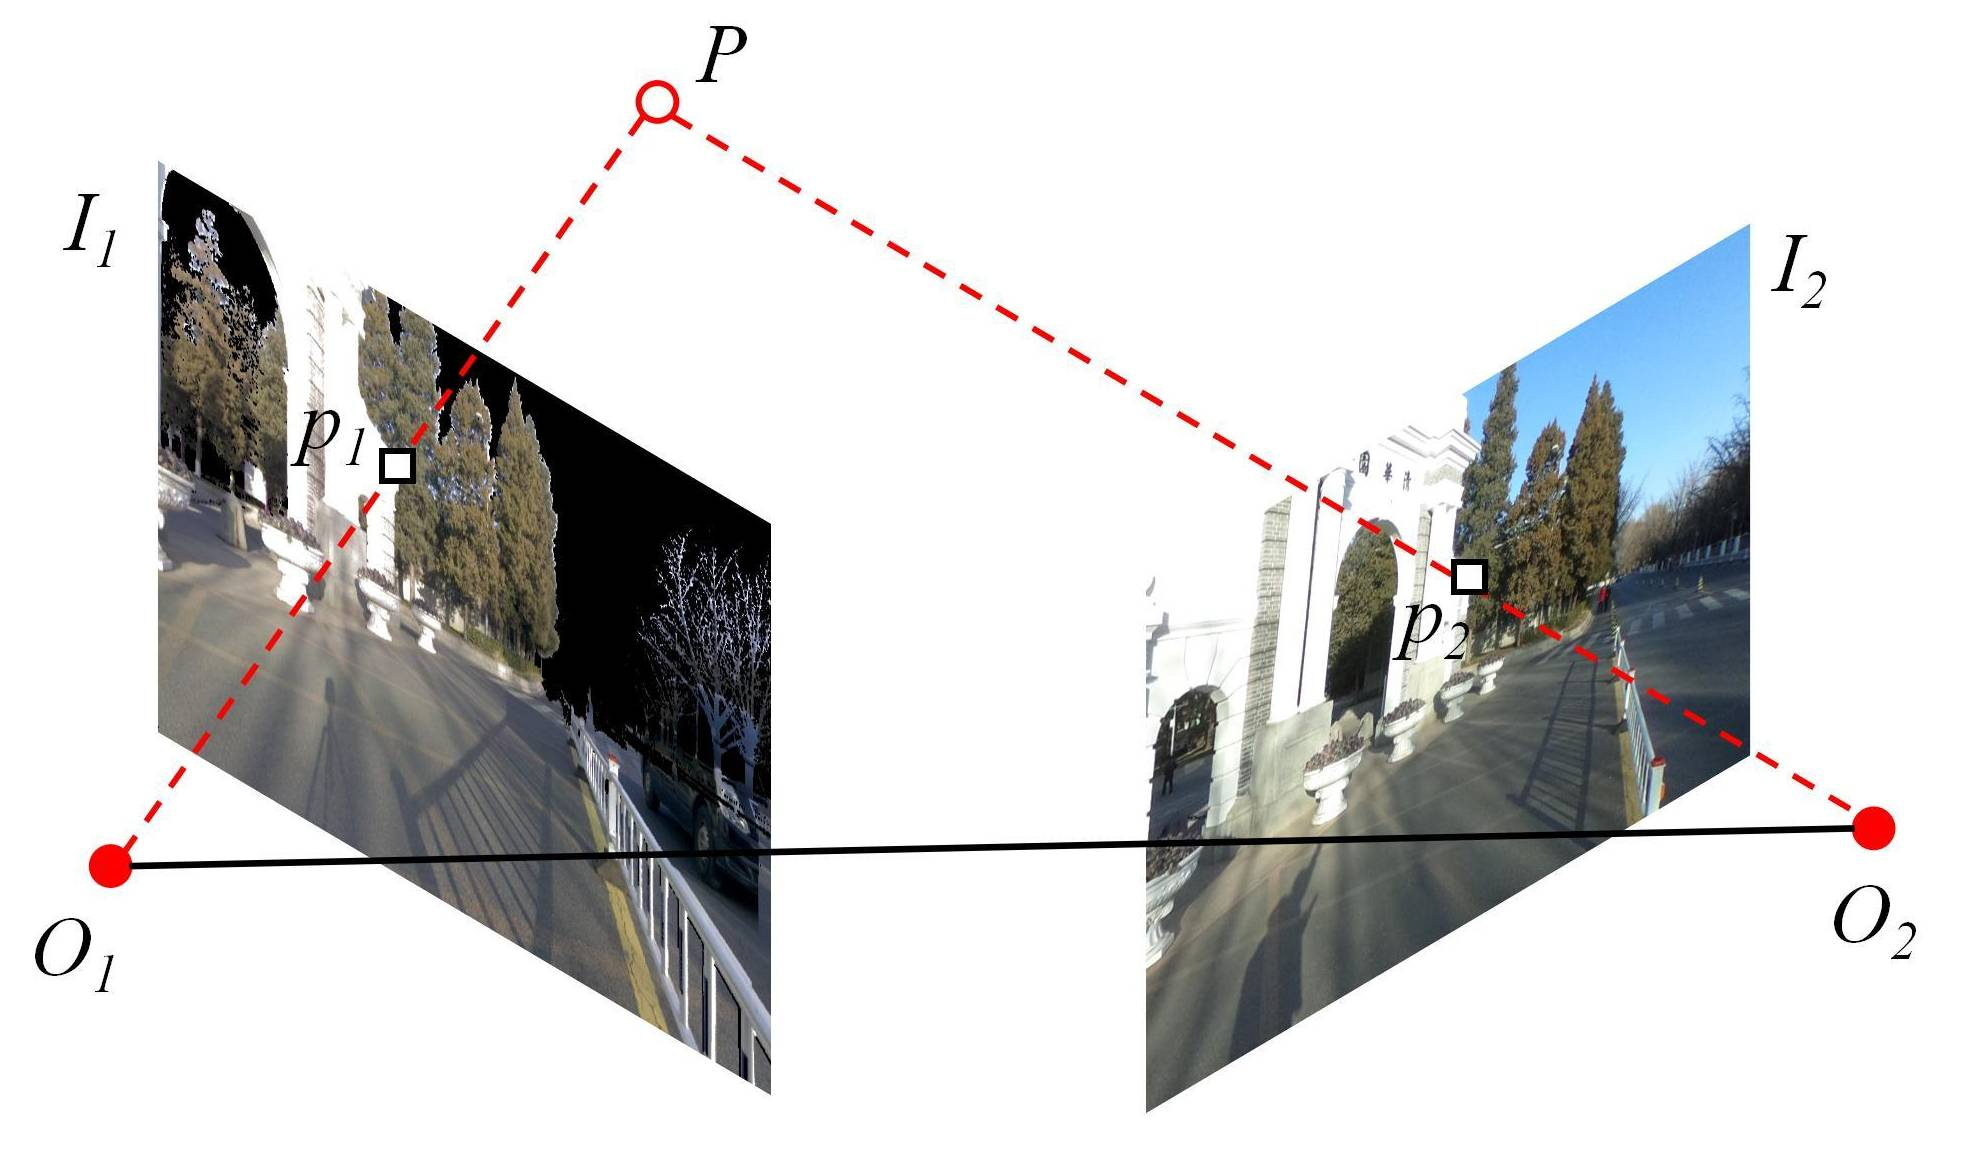
\includegraphics[width=11cm]{epipolar-constraint}
	\caption{对极约束原理示意图}
	\label{epipolar-constraint}
\end{figure}

以图\ref{epipolar-constraint}为例,$I_1$和$I_2$分别是空间中的两帧图像,我们希望求取这两者之间的运动,即求取$\boldsymbol{R}, \boldsymbol{t}$。空间中有一点$\boldsymbol{P}$,坐标为$[X,Y,Z]^T$,根据针孔相机模型,有
\begin{equation}
	\boldsymbol{p}_1=\frac{1}{Z}\boldsymbol{KP}, \quad \boldsymbol{p}_2=\frac{1}{Z}\boldsymbol{K(RP+t)}
\end{equation}
其中$\frac{1}{Z}\boldsymbol{P}$可以看做$\boldsymbol{p}_1$在归一化平面上的坐标,因此不妨令
\begin{equation}
	\boldsymbol{x}_1 = \frac{1}{Z}\boldsymbol{P}, \quad\boldsymbol{x}_2=\frac{1}{Z}(\boldsymbol{R}\boldsymbol{P}+\boldsymbol{t})
\end{equation}

得
\begin{equation}
	\boldsymbol{x}_2=\boldsymbol{R}\boldsymbol{x}_1+\boldsymbol{t}
\end{equation}

上式等号两侧左乘$\boldsymbol{t}\^{}$,$\^{}$符号表示与$\boldsymbol{t}$做外积,得到$\boldsymbol{t}\^{}\boldsymbol{x}_2=\boldsymbol{t}\^{}\boldsymbol{Rx}_1$,然后同时左乘$\boldsymbol{x}_2^T$,得
\begin{equation}
	\boldsymbol{x}_2^T\boldsymbol{t}\^{}\boldsymbol{x}_2=\boldsymbol{x}_2^T\boldsymbol{t}\^{}\boldsymbol{Rx}_1 = 0
\end{equation}

%将$\boldsymbol{p}_1, \boldsymbol{p}_2$带入上式,有
%\begin{equation}
%	\boldsymbol{p}_2^T \boldsymbol{K}^{-T} \boldsymbol{t}\^{} \boldsymbol{R}\boldsymbol{K}^{-1}\boldsymbol{p}_1 = 0
%\end{equation}

定义本质矩阵$\boldsymbol{E}=\boldsymbol{t}\^{}\boldsymbol{R} $,这是一个$3\times 3$的矩阵,因此本文算法分为以下两个步骤:
\begin{enumerate}
	\item 根据匹配的特征点,计算本质矩阵$\boldsymbol{E}$。这一步通常采用8点法\cite{hartley1997defense, longuet1981computer}进行求解,将矩阵$\boldsymbol{E}$的各个元素用线性方程进行表示并求解。
	\item 根据本质矩阵,求取$\boldsymbol{R}, \boldsymbol{t}$。这一步可以采用SVD分解的方法进行恢复\cite{wang2000svd}。
\end{enumerate}

\subsection{定位实验}
\textbf{1.单帧图像定位实验}

本文利用图\ref{sosnet-match-result}的特征匹配结果进行了单时刻的定位。由于不可避免地由于参数设置不能很好地处理不同场景的图像特征,SOSNet的匹配结果中也有可能产生误匹配的现象,因此为了减小错误匹配对结果的影响,类似点云配准的操作,本文采用了RANSAC方法,随机的从匹配点中选择八对特征点进行本质矩阵的估计,并选择在未被选中的点中拟合效果最好的一次作为最终模型结果。

计算得到的本质矩阵为
\begin{equation*}
	\boldsymbol{E} = 
	\begin{bmatrix}
		-0.021 & 0.467 & -0.179\\
		-0.472 & -0.030 & 0.492\\
		0.210 & -0.489 & -0.003
	\end{bmatrix}
\end{equation*}

从本质矩阵中恢复出从点云平面图到全景平面图之间的相机运动为
\begin{equation*}
	\boldsymbol{R} = 
	\begin{bmatrix}
		0.999 & 0.051 & 0.015 \\
		-0.051 & 0.999 & 0.012\\
		-0.015 & -0.013 & 1.000
	\end{bmatrix}
\end{equation*}
\begin{equation*}
	\boldsymbol{t}=[-0.706, -0.261, -0.659]^T
\end{equation*}

由此根据$\boldsymbol{t}$,便得到了在点云坐标系下的相机坐标。

\textbf{2.多帧连续图像定位实验}

与单帧图像类似,本文在基于连续视频的定位上进行了实验,这次实验场景选在了室内,离线地图是图\ref{reg-result-indoor}中合并的地图,对于其中的三个子点云,分别以它们的中心为虚拟观测,选择了4个角度生成平面合成图,因此总共得到了12张离线子地图,以及12个它们对应的位置和视角信息。一个连续视频流的定位问题可以分解为一下两个步骤,第一是能够在场景中不依赖先验条件的情况下初始化定位,第二是根据上一帧的定位信息以及当前数据更新当前时刻的位置信息。本文按照以下算法处理这两个问题:

\textbf{初始化定位} \quad 选定水平视场角和垂直视场角,将全景图沿某一方向进行投影,分别在12张离线地图图像中搜索特征匹配,若某一张图片特征匹配数大于阈值,则以该图片对应的测站作为基准,估计其到全景相机的运动,得到初始化坐标;若所有离线子地图均无法产生足够的有效配对,则表示全景图的投影方向可能特征不够明显,更换投影方向重复上述操作,直至产生足够多有效配对为止,最终得到初始的位置$\boldsymbol{t}$。

\textbf{基于先验信息的位置更新} \quad 对于全景相机,保持与上一帧的投影方向不变;由于知道了相机在上一帧中对于离线地图的旋转角和平移向量,因此选择距离上一帧位置最近的测站作为基准,在其中的4张离线地图图像中选择视角与全景投影视角相差最小的合成图像进行配对,从而更新相机的位置和角度信息;若无法产生有效配对,则更换全景投影方向,并依次与最近测站中的4张平面图进行配对,最终得到当前时刻相机的位置和旋转角。

利用以上算法,以$544\times 960$的分辨率、30fps的帧率在室内场景中拍摄一段20秒左右的全景视频,同时每隔5帧更新一次位置信息,因此相当于对120张时序图像进行了定位,其结果如图\ref{localization-result}所示,其中黄色线条为相机的运动轨迹,为了更好地看清建图及定位效果,对屋顶部分进行了去除。

\begin{figure}
	\centering
	\subcaptionbox{俯视图}	{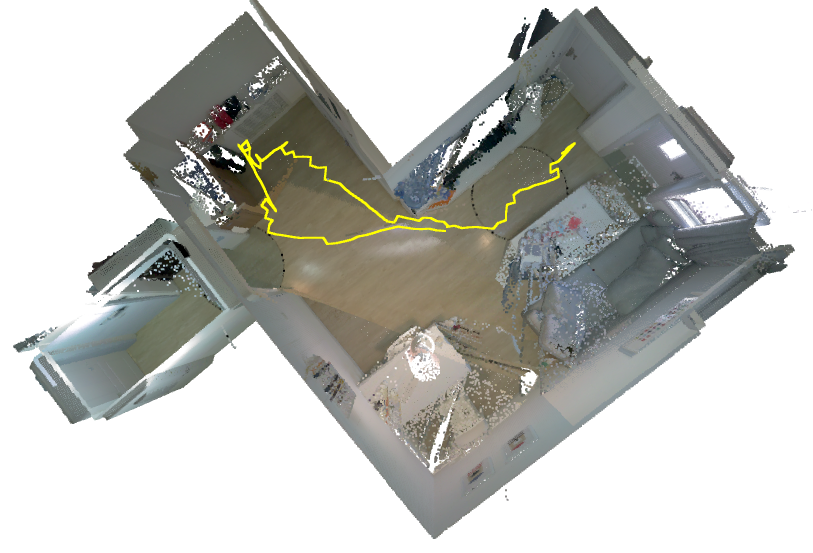
\includegraphics[width=13cm]{localization-result-1}}\\
	\subcaptionbox{侧视图} {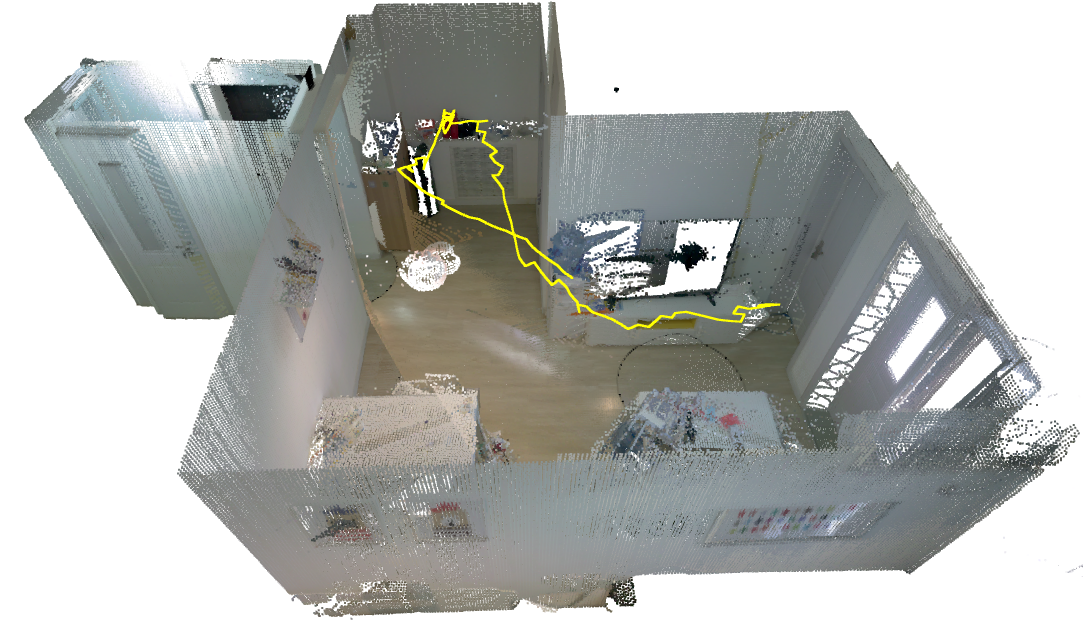
\includegraphics[width=13cm]{localization-result-2}}
	\caption{室内场景定位结果图}
	\label{localization-result}
\end{figure}

\section{本章小结}
本章解决了基于离线点云地图的视觉定位的问题。在整体框架上来看,本章将3D-2D匹配问题转换成了2D-2D匹配问题,在离线地图中生成局部视点,合成某一视角的平面图像,并利用基于图像二阶相似性的SOSNet网络对离线图像与在线图像之间进行特征匹配,最后通过对极约束求得两者的相对位置,即获得相机的六自由度。

同时,本章也在室外和室内分别进行了单帧图像的定位与图像序列的定位实验,实验结果均证明了本文提到的定位方法的可行性。






